%%%%%%%%%%%%%%%%%%%%%%%%%%  ltexpprt.tex  %%%%%%%%%%%%%%%%%%%%%%%%%%%%%%%%
%
% This is ltexpprt.tex, an example file for use with the SIAM LaTeX2E
% Preprint Series macros. It is designed to provide double-column output.
% Please take the time to read the following comments, as they document
% how to use these macros. This file can be composed and printed out for
% use as sample output.

% Any comments or questions regarding these macros should be directed to:
%
%                 Donna Witzleben
%                 SIAM
%                 3600 University City Science Center
%                 Philadelphia, PA 19104-2688
%                 USA
%                 Telephone: (215) 382-9800
%                 Fax: (215) 386-7999
%                 e-mail: witzleben@siam.org


% This file is to be used as an example for style only. It should not be read
% for content.

%%%%%%%%%%%%%%% PLEASE NOTE THE FOLLOWING STYLE RESTRICTIONS %%%%%%%%%%%%%%%

%%  1. There are no new tags.  Existing LaTeX tags have been formatted to match
%%     the Preprint series style.
%%
%%  2. You must use \cite in the text to mark your reference citations and
%%     \bibitem in the listing of references at the end of your chapter. See
%%     the examples in the following file. If you are using BibTeX, please
%%     supply the bst file with the manuscript file.
%%
%%  3. This macro is set up for two levels of headings (\section and
%%     \subsection). The macro will automatically number the headings for you.
%%
%%  5. No running heads are to be used for this volume.
%%
%%  6. Theorems, Lemmas, Definitions, etc. are to be double numbered,
%%     indicating the section and the occurence of that element
%%     within that section. (For example, the first theorem in the second
%%     section would be numbered 2.1. The macro will
%%     automatically do the numbering for you.
%%
%%  7. Figures, equations, and tables must be single-numbered.
%%     Use existing LaTeX tags for these elements.
%%     Numbering will be done automatically.
%%
%%  8. Page numbering is no longer included in this macro.
%%     Pagination will be set by the program committee.
%%
%%
%%%%%%%%%%%%%%%%%%%%%%%%%%%%%%%%%%%%%%%%%%%%%%%%%%%%%%%%%%%%%%%%%%%%%%%%%%%%%%%



\documentclass[twoside,leqno,twocolumn]{article}
\usepackage{ltexpprt}

%jing
\usepackage{graphicx}
\usepackage{balance}  % for  \balance command ON LAST PAGE  (only there!)
%
\usepackage{amsmath,amssymb}
%\usepackage[ruled]{algorithm2e}
\usepackage{xcolor}
\usepackage{caption2}
%\usepackage{verbatim}
\usepackage{url}
%%wj\usepackage{paralist}
%%wj\usepackage{lstautogobble}
%%wj\usepackage{listings}
%
%\usepackage{subcaption}
\usepackage{amsmath}
%\usepackage{bbold}
\usepackage{subfigure}
%\usepackage{enumitem}
\usepackage{textcomp}
%\usepackage{graphicx}
\usepackage{multirow}
\usepackage{comment}
\usepackage{algorithm}
\usepackage{algpseudocode}
\usepackage{booktabs}
\usepackage{CJK}

\begin{document}
\begin{CJK*}{GBK}{song}


%jing
\newtheorem{definition}{Definition}
\newtheorem{problem}{Problem}
%\newtheorem{theorem}{Theorem}
\newtheorem{remark}{Remark}
%\newtheorem{lemma}[theorem]{Lemma}
%\newtheorem{corollary}[theorem]{Corollary}
%
%\newcommand{\exa}[2]{{\tt\begin{tabbing}\hspace{#1}\=\+\kill #2\end{tabbing}}}
\newcommand{\sys}{\uppercase{G}\lowercase{ru}\uppercase{B}\lowercase{a}}
\newcommand{\tbc}{\textcolor{blue}{[To Be Completed]}}
\newcommand{\refe}{\textcolor{blue}{[reference]}}
\newcommand{\retg}{retweeting}
\newcommand{\retgs}{retweetings}
\newcommand{\Retg}{Retweeting}
\newcommand{\retd}{retweeted}
\newcommand{\ret}{retweet}
\newcommand{\tw}{tweet}
\newcommand{\twd}{tweeted}
\newcommand{\twg}{tweeting}
\newcommand{\od}{Euclidean distance}
\newcommand{\hd}{Hamiltonian distance}
\newcommand{\gd}{GruBa Distance}
%%jing


%\setcounter{chapter}{2} % If you are doing your chapter as chapter one,
%\setcounter{section}{3} % comment these two lines out.

\newcommand{\stitle}[1]{\vspace{0.5ex}\noindent{\bf #1}}
\newcommand{\etitle}[1]{\vspace{0.5ex}\noindent{\em \underline{#1}}}
\newcommand{\stab}{\rule{0pt}{8pt}\\[-2ex]}
\newcommand{\sstab}{\rule{0pt}{8pt}\\[-2.5ex]}
\newcommand{\beihang}{SKLSDE Lab, Beihang University, China. Email: \{zhujh@act., mashuai, zhanghui@act., hucm@\}buaa.edu.cn, wjseawind@gmail.com}
%\newcommand{\beihang}{SKLSDE Lab, Beihang University, China. Email: \{zhujh@act., mashuai, zhanghui@act., hucm@\}buaa.edu.cn}
\newcommand{\ackfunding}{Supported by NSFC (U1636210, 61421003, 61403090, U1636123), Beijing Advanced Innovation Center for Big Data and Brain Computing.}

\begin{comment}
\title{\Large Incorporating User Grouping into \Retg{} Behavior Modeling}
\author{Jinhan Zhu\thanks{\beihang}\hspace{2ex} Shuai Ma$^{\dag}$\hspace{2ex} Jing Wang$^{\dag}$\hspace{2ex} Hui Zhang$^{\dag}$\hspace{2ex} Chunming Hu$^{\dag}$\\
\and
\hspace{-2ex}Xiong Li\thanks{National Computer Network Emergency Response Technical Team/Coordination Center of China. Email:li.xiong@foxmail.com}}
\date{}	

\date{}	
\end{comment}

\title{\Large Incorporating User Grouping into \Retg{} Behavior Modeling\\ Supplementary Material}
\author{Jinhai Zhu\thanks{\beihang}
\hspace{2ex} Shuai Ma$^{*}$
\hspace{2ex} Jing Wang$^{*}$
\hspace{2ex} Hui Zhang$^{*}$
\hspace{2ex} Chunming Hu$^{*}$
\hspace{2ex} Xiong Li\thanks{National Computer Network Emergency Response Technical Team/Coordination Center of China.  Email: li.xiong@foxmail.com}}


\date{}	

\maketitle


%\footnote[1]{\footnotesize{\textbf{SKLSDE Lab, Beihang University, China. Email: \{zhujh@act., mashuai, zhanghui@act., hucm@\}buaa.edu.cn., wjseawind@gmail.com}}}}

% Copyright Statement
% When submitting your final paper to a SIAM proceedings, it is requested that you include
% the appropriate copyright in the footer of the paper.  The copyright added should be
% consistent with the copyright selected on the copyright form submitted with the paper.
% Please note that "20XX" should be changed to the year of the meeting.

% Default Copyright Statement
%\fancyfoot[R]{\footnotesize{\textbf{Copyright \textcopyright\ 2018 by SIAM\\ Unauthorized reproduction of this article is prohibited}}}

% Depending on which copyright you agree to when you sign the copyright form, the copyright
% can be changed to one of the following after commenting out the default copyright statement
% above.

%\fancyfoot[R]{\footnotesize{\textbf{Copyright \textcopyright\ 20XX\\
%Copyright for this paper is retained by authors}}}

%\fancyfoot[R]{\footnotesize{\textbf{Copyright \textcopyright\ 20XX\\
%Copyright retained by principal author's organization}}}


%\pagenumbering{arabic}
%\setcounter{page}{1}%Leave this line commented out.


\section*{Appendix: Extra Experiments}
\label{sec:appendix}

%\subsection{Case Study for Feature Extraction}
\begin{figure*}
  \centering
  \subfigure[]{
  \label{fig:subfig1:fig11}
      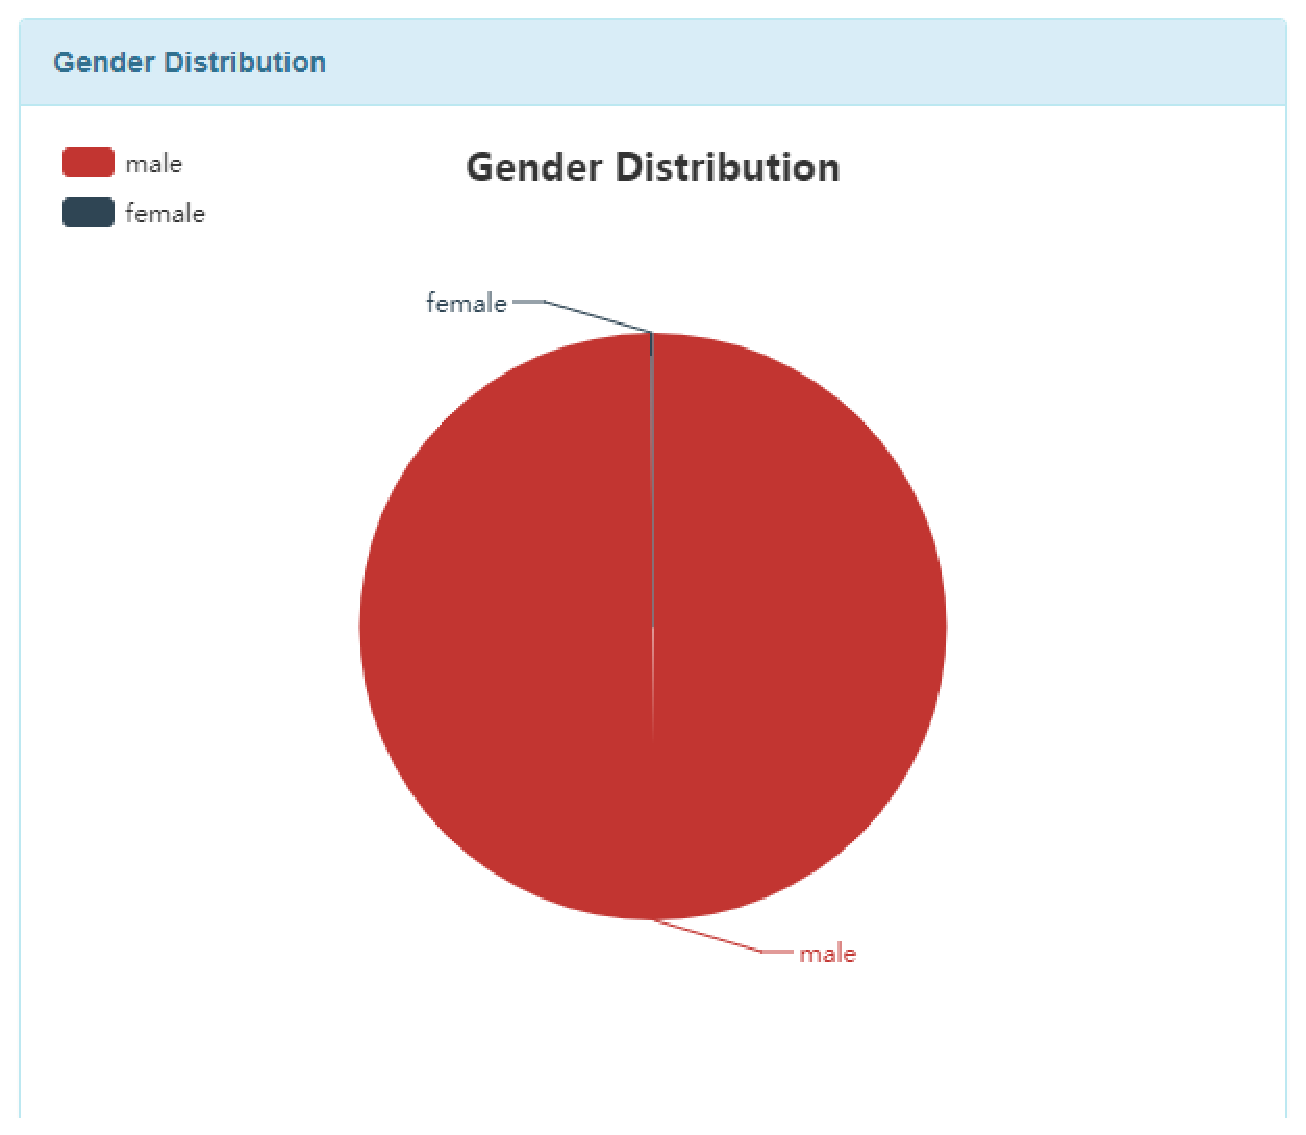
\includegraphics[width=0.23\textwidth]{IMAGE/group-images/11.eps}}
  \subfigure[]{
  \label{fig:subfig1:fig12}
      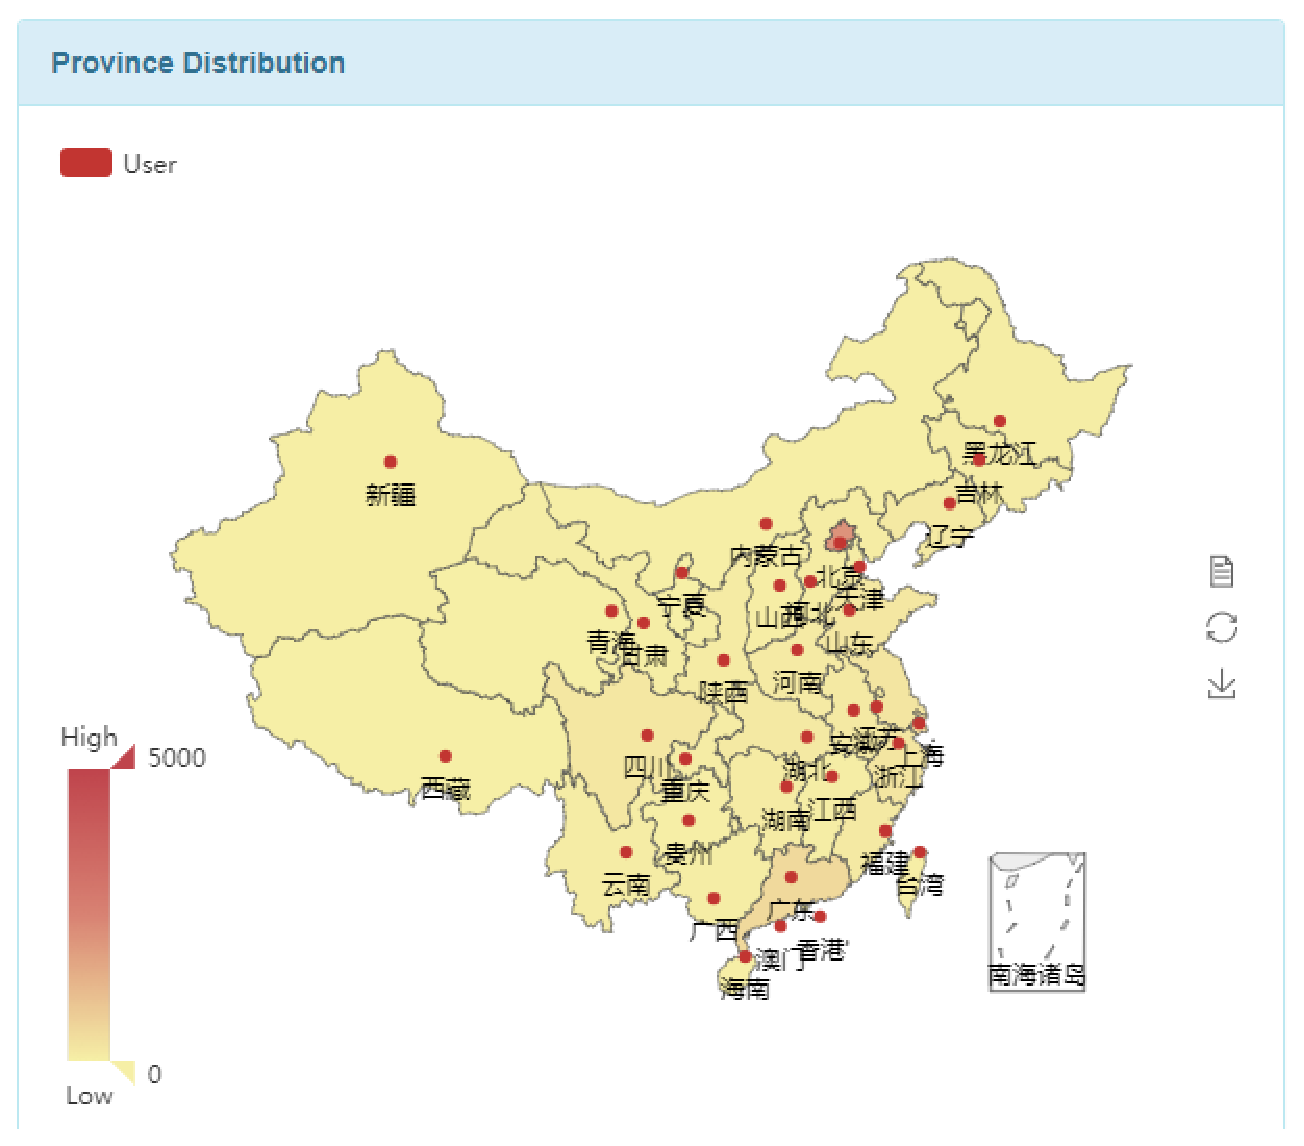
\includegraphics[width=0.23\textwidth]{IMAGE/group-images/12.eps}}
  \subfigure[]{
  \label{fig:subfig1:fig13}
      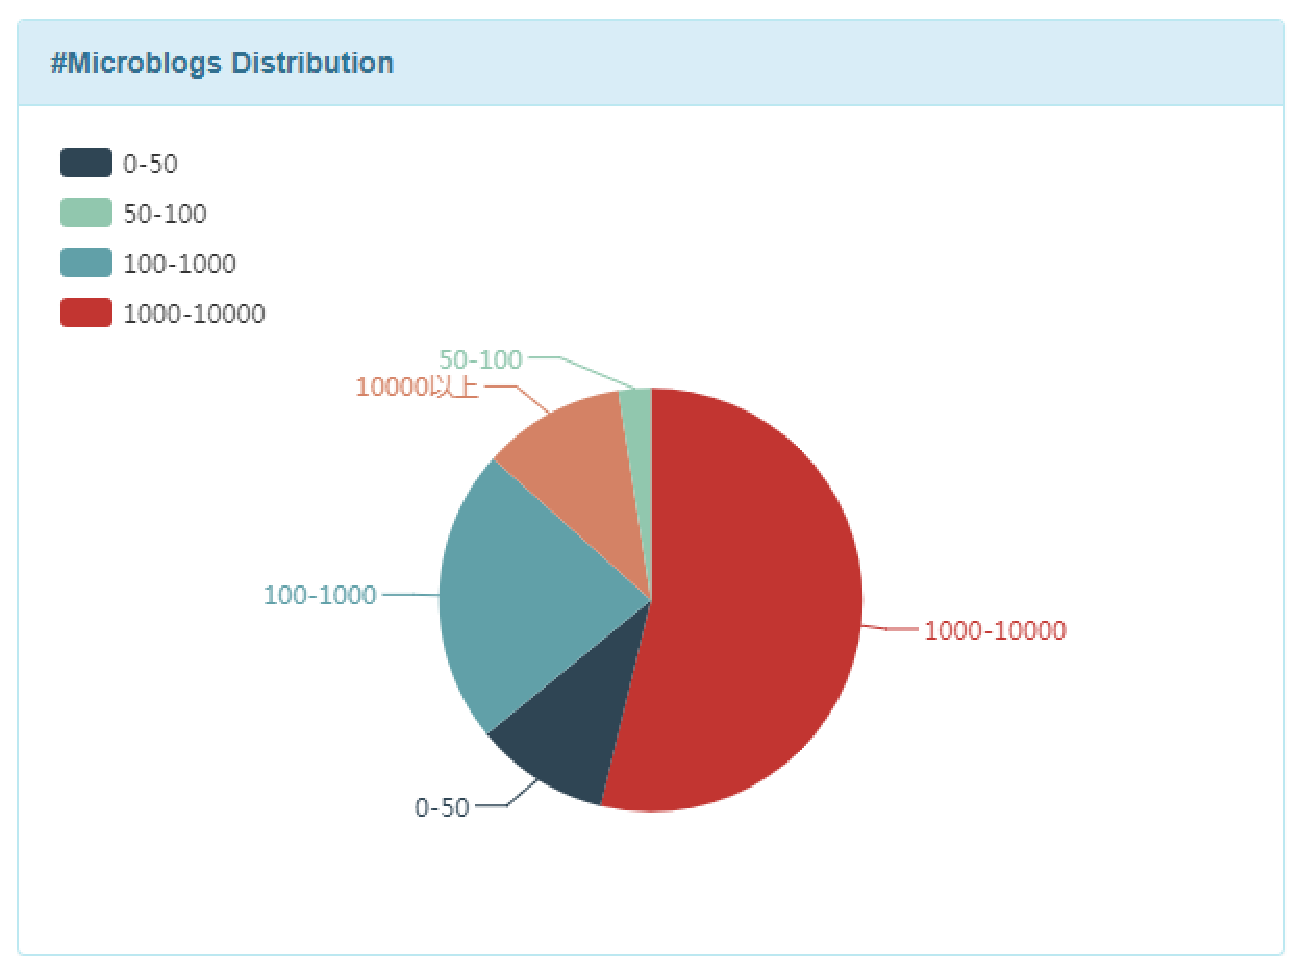
\includegraphics[width=0.23\textwidth]{IMAGE/group-images/13.eps}}
  \subfigure[]{
  \label{fig:subfig1:fig14}
      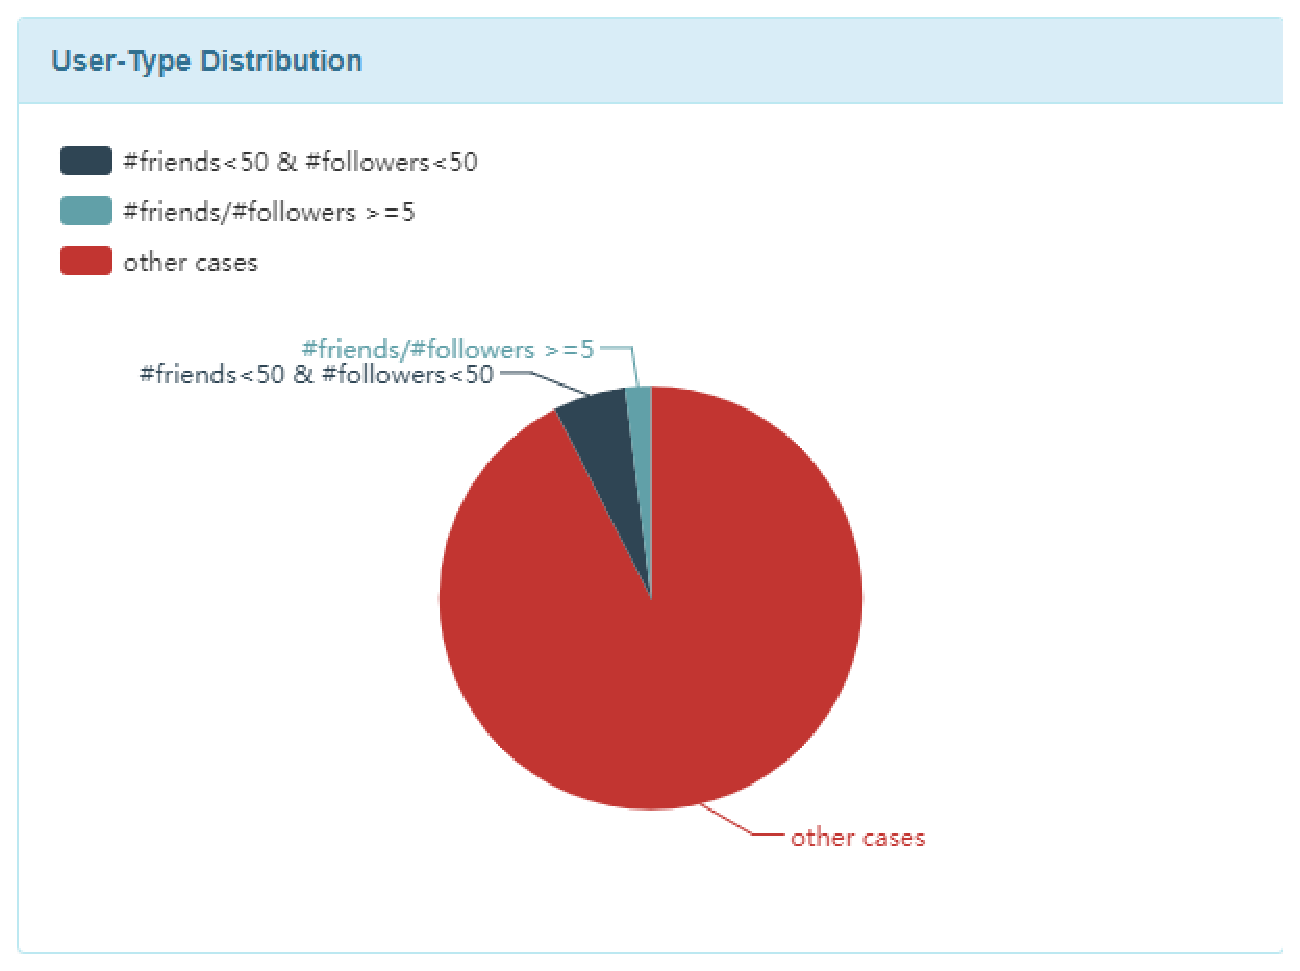
\includegraphics[width=0.23\textwidth]{IMAGE/group-images/14.eps}}
  \subfigure[]{
  \label{fig:subfig1:fig15}
      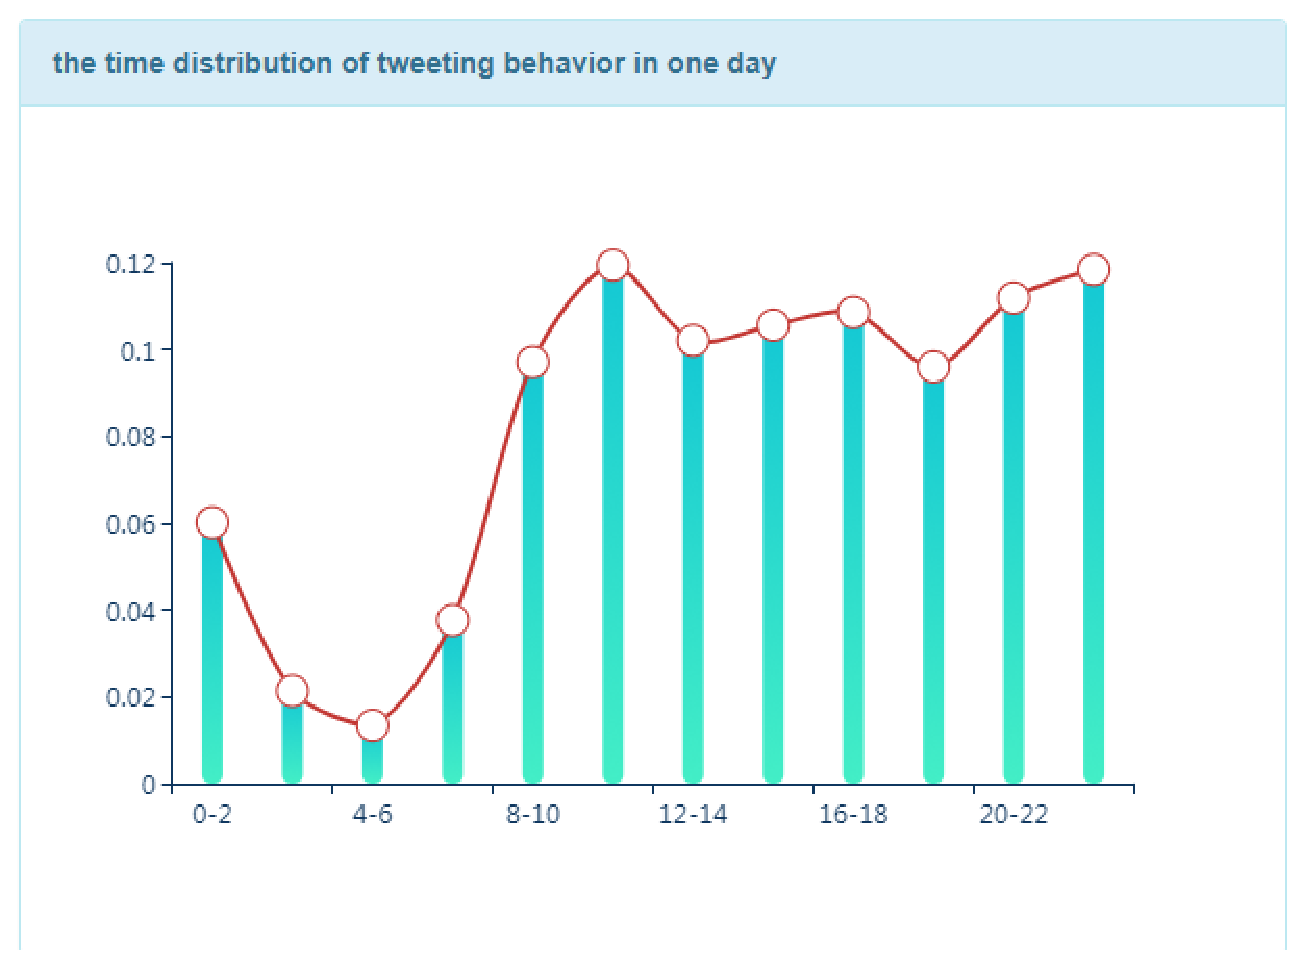
\includegraphics[width=0.23\textwidth]{IMAGE/group-images/15.eps}}
  \subfigure[]{
  \label{fig:subfig1:fig16}
      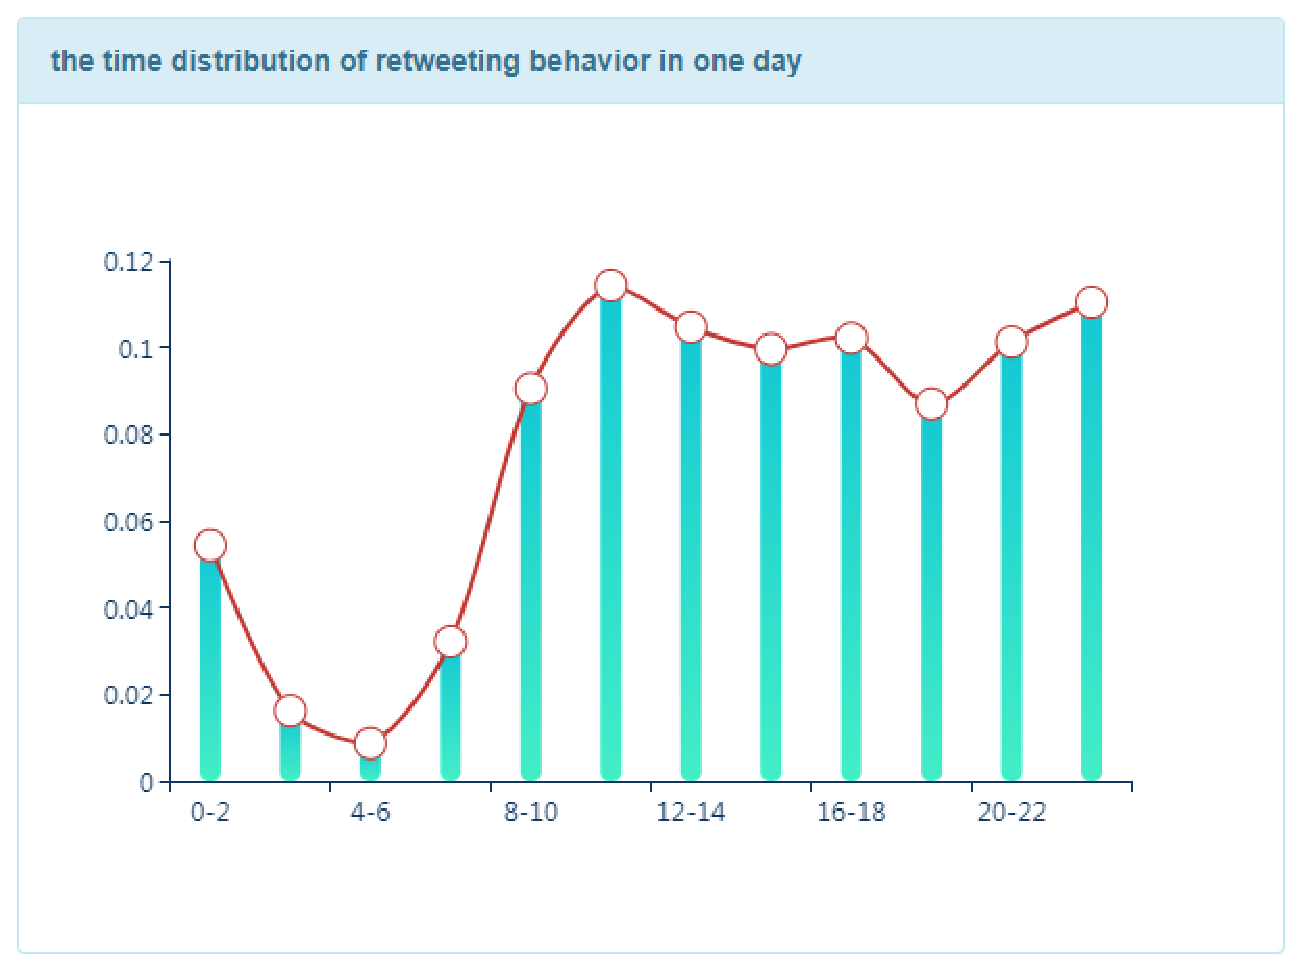
\includegraphics[width=0.23\textwidth]{IMAGE/group-images/16.eps}}
  \subfigure[]{
  \label{fig:subfig1:fig17}
      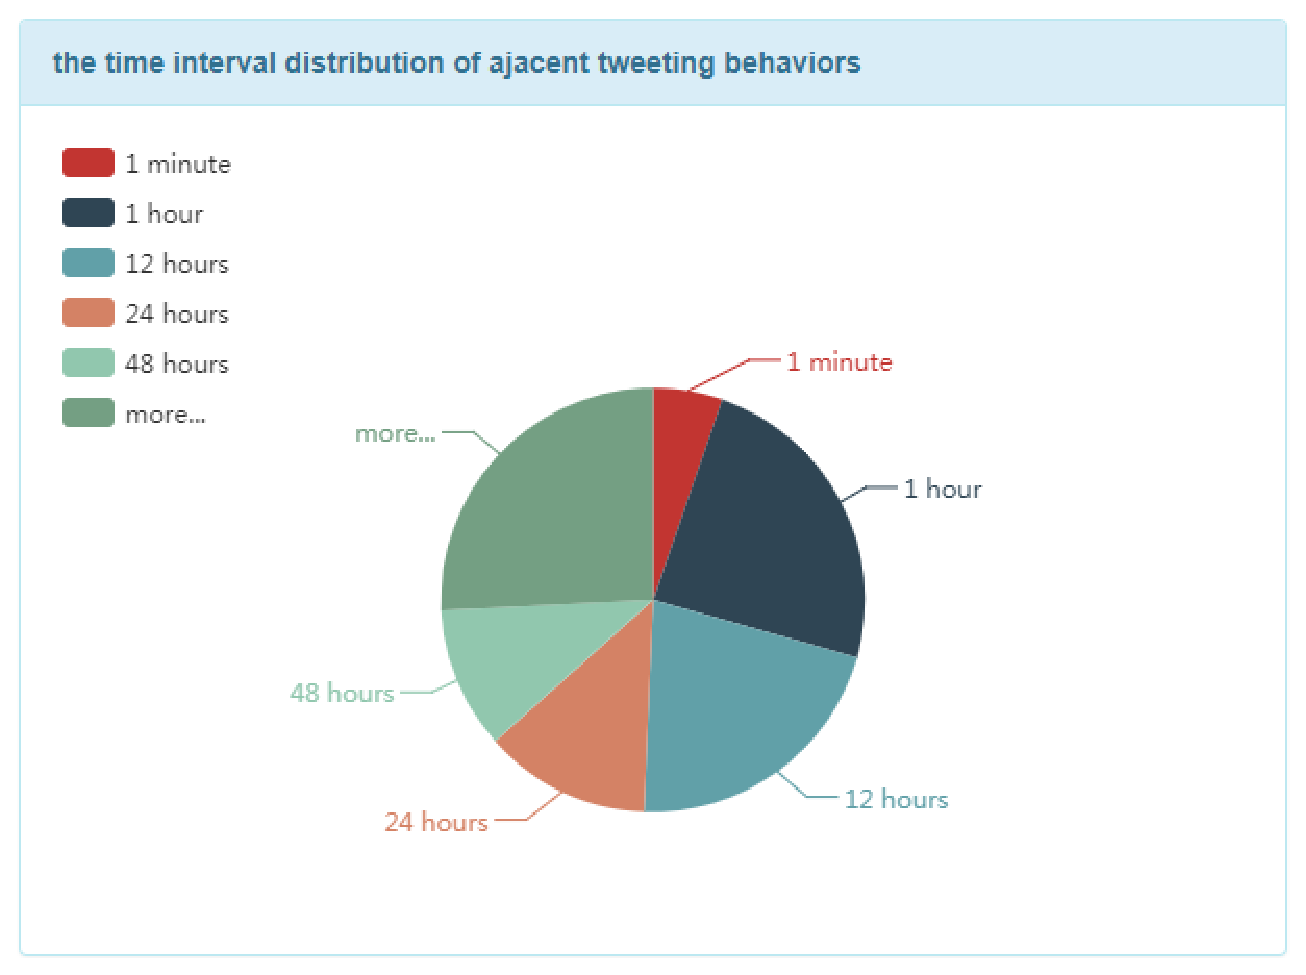
\includegraphics[width=0.23\textwidth]{IMAGE/group-images/17.eps}}
  \subfigure[]{
  \label{fig:subfig1:fig18}
      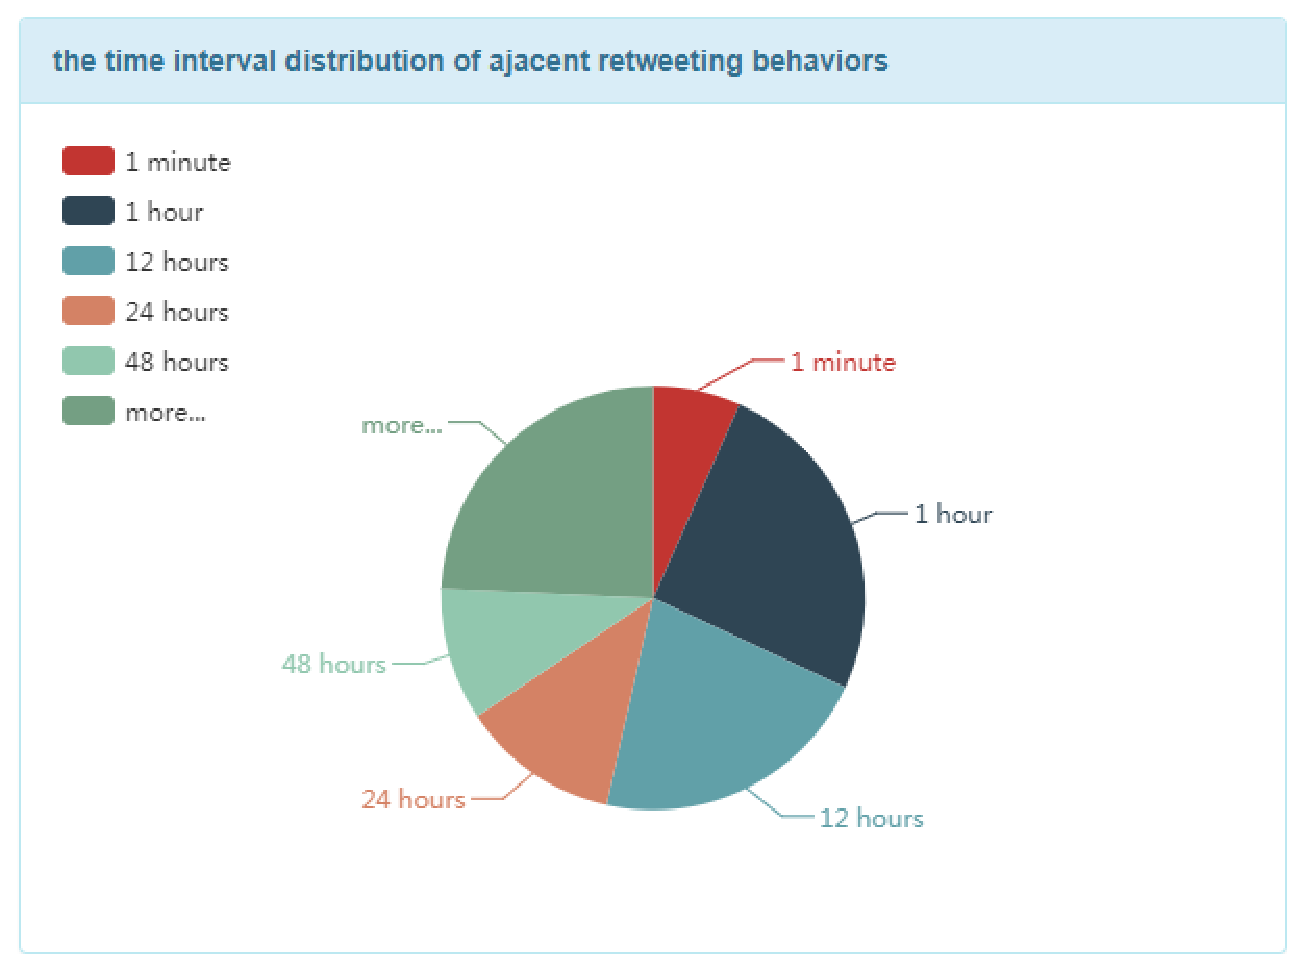
\includegraphics[width=0.23\textwidth]{IMAGE/group-images/18.eps}}
  \subfigure[]{
  \label{fig:subfig1:fig19}
      
\includegraphics[width=0.23\textwidth]{IMAGE/group-images/19.eps}}
  \caption{The Statistics of User Group One}
  \label{fig:subfig1} %% label for entire figure
\end{figure*}

\subsection*{Exp-5: Case Study for User Clustering}

In this section, we show the results of our system \sys{} for User Clustering. We carefully analyzed the statistical information of four groups obtained from user clustering.

\stab(1) Most users of group one are male (as shown in Sub-Fig. \ref{fig:subfig1:fig11}), and Sub-Fig. \ref{fig:subfig1:fig12} shows that they are mainly in Beijing(����). The amount of their followees is mostly similar as their followers (as shown in Sub-Fig. \ref{fig:subfig1:fig14}). The most active time of this group is mainly between 10 am and 12 am (as shown in Sub-Fig. \ref{fig:subfig1:fig15} and \ref{fig:subfig1:fig16}).

\stab(2) Mostly users of group two are  female (as shown in Sub-Fig. \ref{fig:subfig2:fig21}) and are also mainly in Beijing (����) (shown as Sub-Fig. \ref{fig:subfig2:fig22}). Similar to group one, most of them have followees close to followers (as shown in Sub-Fig. \ref{fig:subfig2:fig24}). The most active time of this group is mainly between 10 pm and 12 pm (as shown in Sub-Fig. \ref{fig:subfig2:fig25} and \ref{fig:subfig2:fig26}).

\stab(3) Most users of group three are male (as shown in Sub-Fig. \ref{fig:subfig3:fig31}). They come from a wide range of provinces (as shown in Sub-Fig. \ref{fig:subfig3:fig32}). Most of them have number of followers far more than followees (as shown in Sub-Fig. \ref{fig:subfig3:fig34}). The most active time of this group is mainly in 10-12 am and 10-12 pm (as shown in Sub-Fig. \ref{fig:subfig3:fig35} and \ref{fig:subfig3:fig36}).

\stab(4) Most users of group four are female (as shown in Sub-Fig. \ref{fig:subfig4:fig41}), and they come from a wide range of provinces just as group three (as shown in Sub-Fig. \ref{fig:subfig4:fig42}). Most of these users have the amount  of followers far more than followees (as shown in Sub-Fig. \ref{fig:subfig4:fig44}). And the most active time of these users is mainly between 10 pm and 12 pm (as shown in Sub-Fig. \ref{fig:subfig4:fig45} and \ref{fig:subfig4:fig46}).

According to Sub-Figs. \ref{fig:subfig1:fig13}, \ref{fig:subfig2:fig23}, \ref{fig:subfig3:fig33} and \ref{fig:subfig4:fig43},
the number distribution of microblogs for four groups is similar with each other.
We visualize each group's long-term interest expressed as words cloud (shown in Sub-Figs. \ref{fig:subfig1:fig19}, \ref{fig:subfig2:fig29}, \ref{fig:subfig3:fig39} and \ref{fig:subfig4:fig49}). As we can see, group one and group three have similar interests.



\begin{figure*}
  \centering
  \subfigure[]{
  \label{fig:subfig2:fig21}
      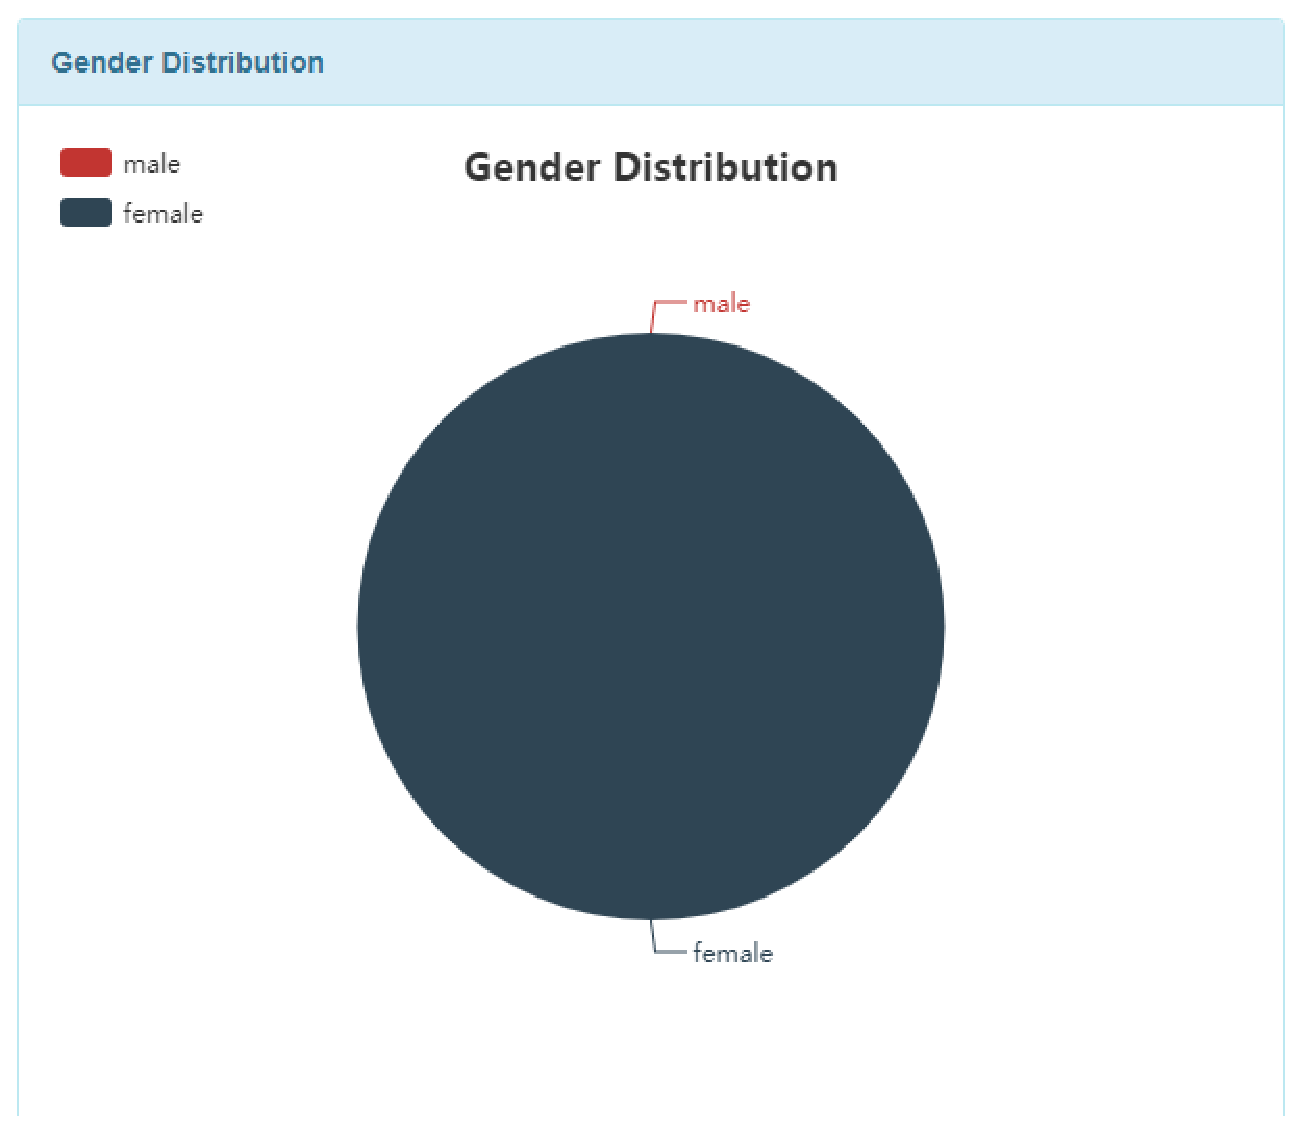
\includegraphics[width=0.23\textwidth]{IMAGE/group-images/21.eps}}
  \subfigure[]{
  \label{fig:subfig2:fig22}
      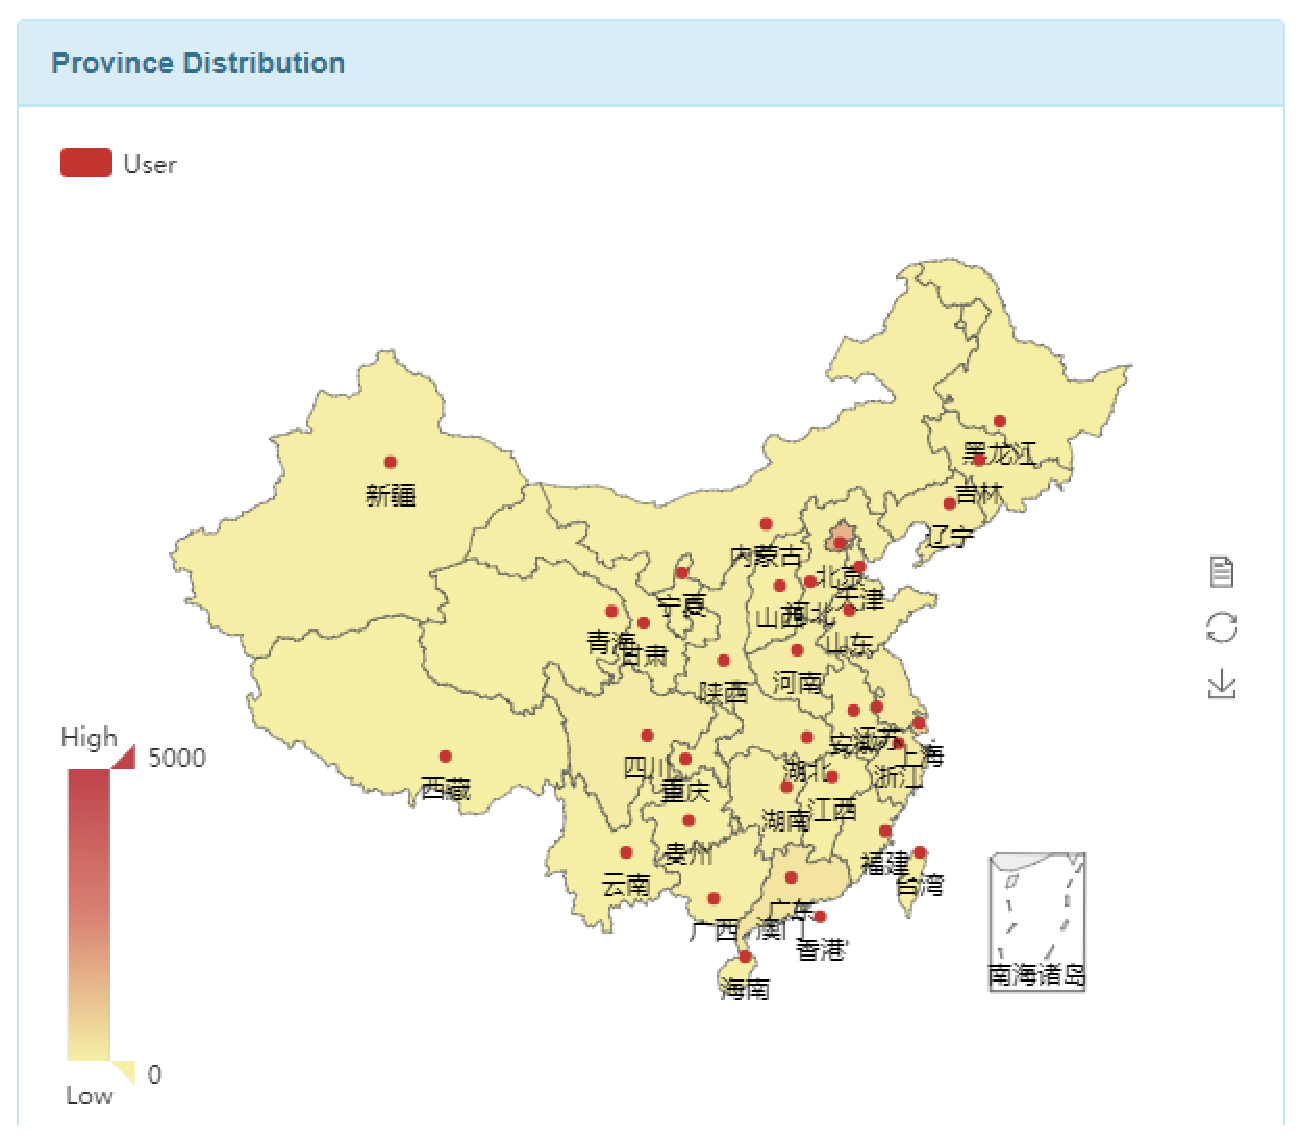
\includegraphics[width=0.23\textwidth]{IMAGE/group-images/22.eps}}
  \subfigure[]{
  \label{fig:subfig2:fig23}
      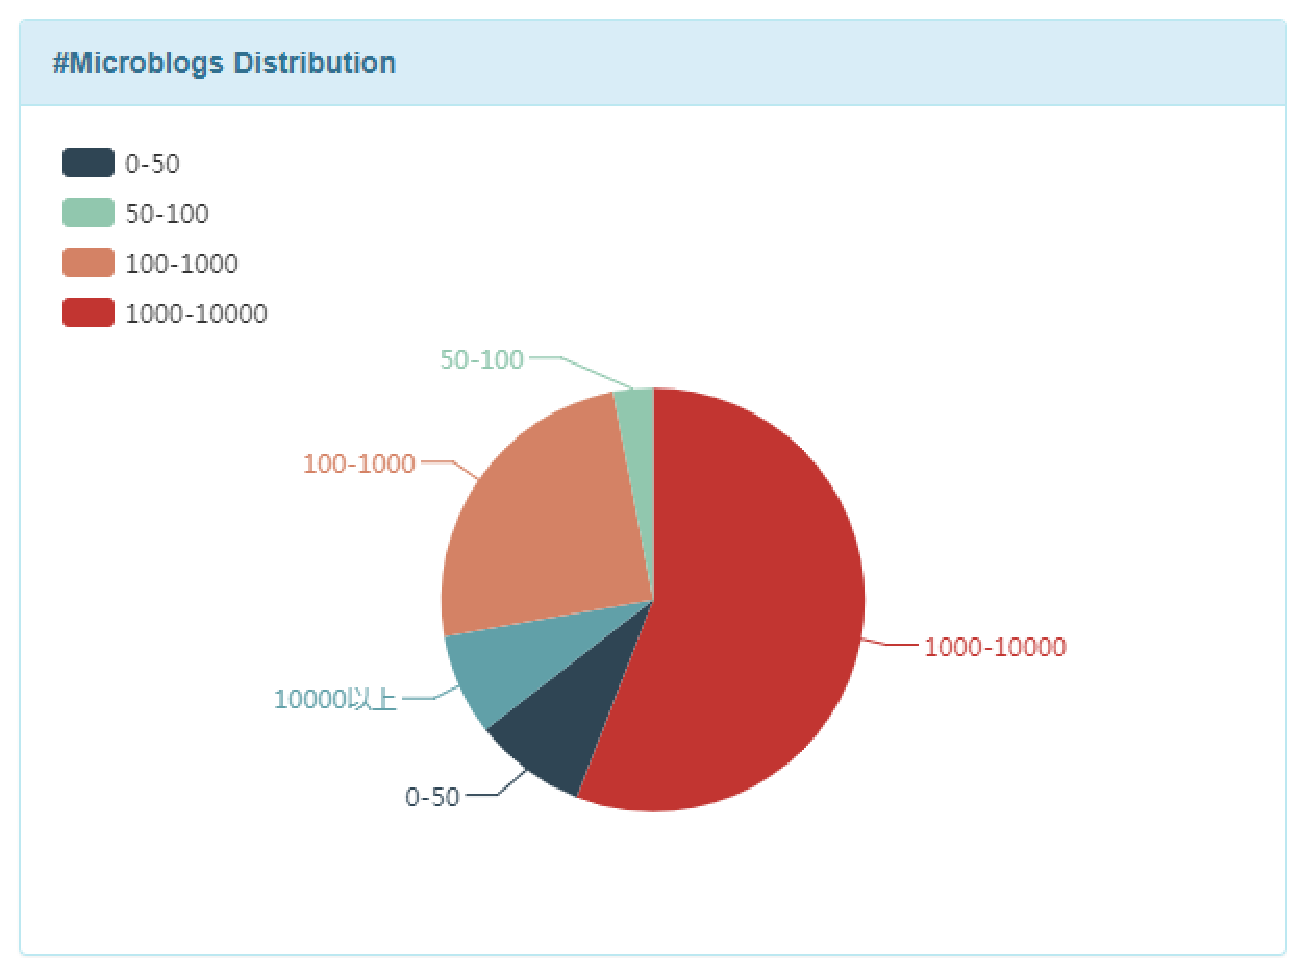
\includegraphics[width=0.23\textwidth]{IMAGE/group-images/23.eps}}
  \subfigure[]{
  \label{fig:subfig2:fig24}
      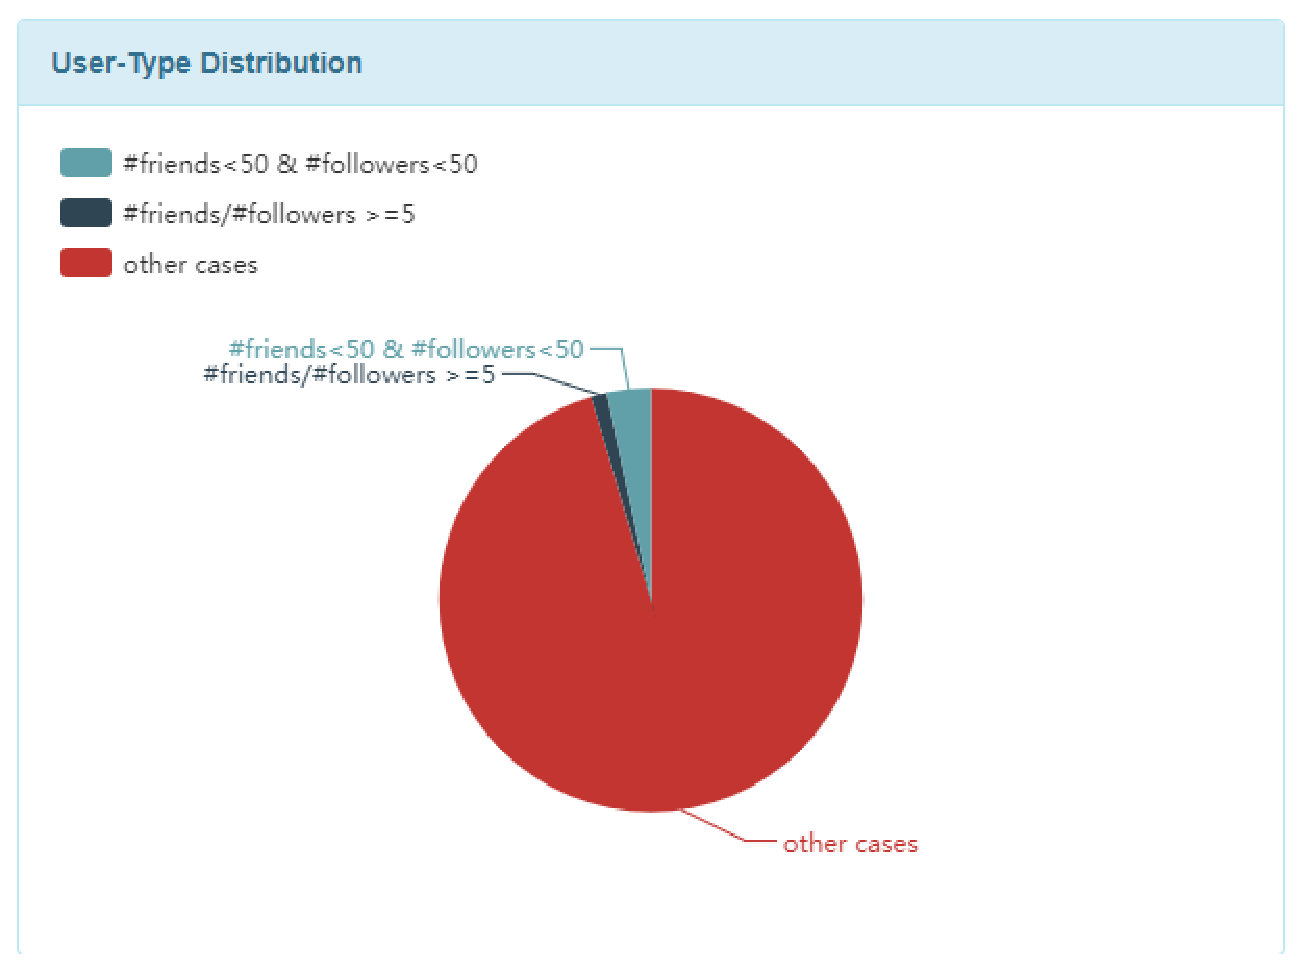
\includegraphics[width=0.23\textwidth]{IMAGE/group-images/24.eps}}
  \subfigure[]{
  \label{fig:subfig2:fig25}
      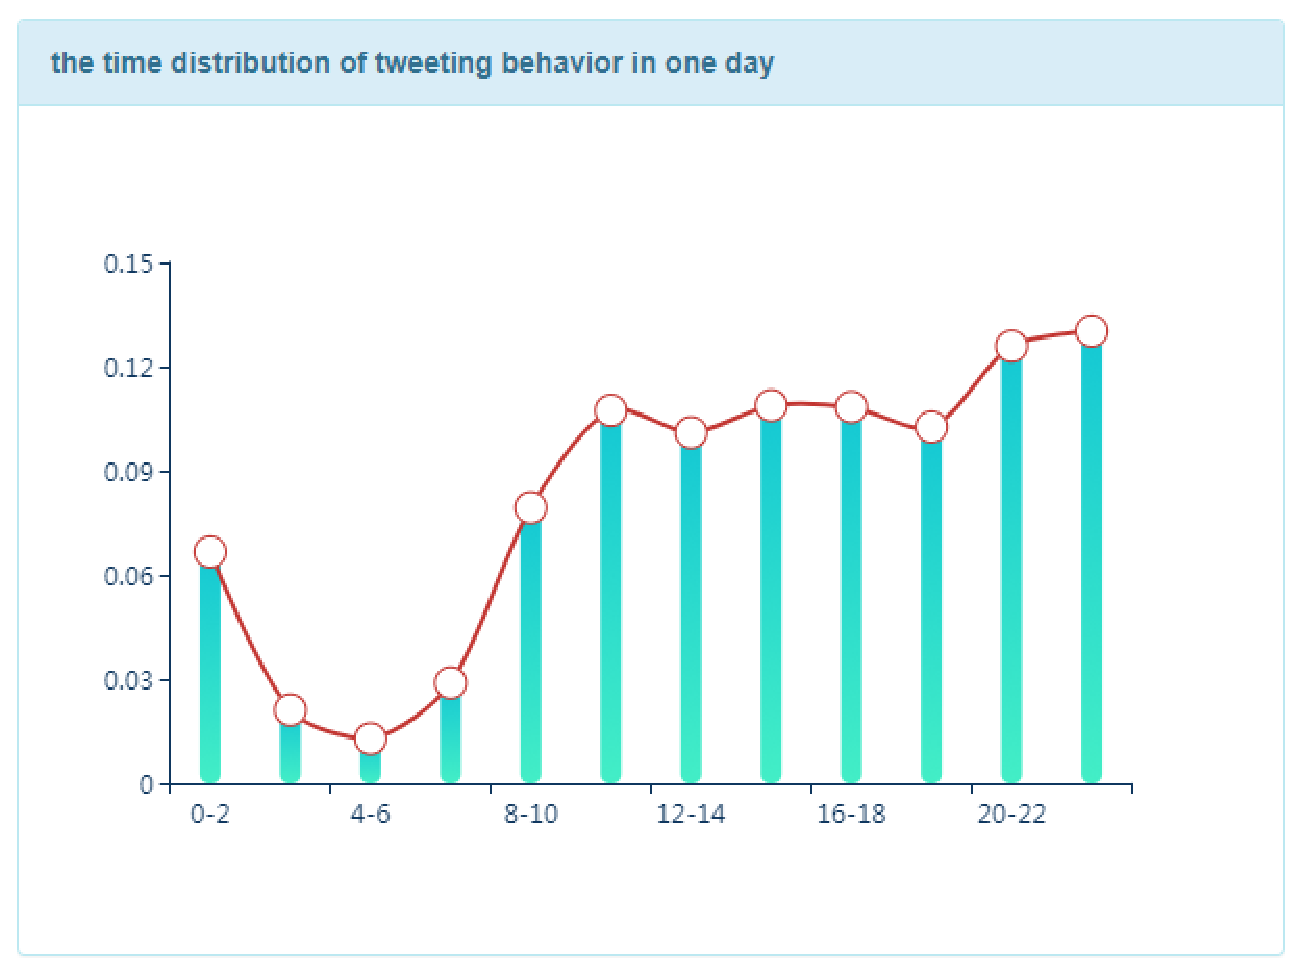
\includegraphics[width=0.23\textwidth]{IMAGE/group-images/25.eps}}
  \subfigure[]{
  \label{fig:subfig2:fig26}
      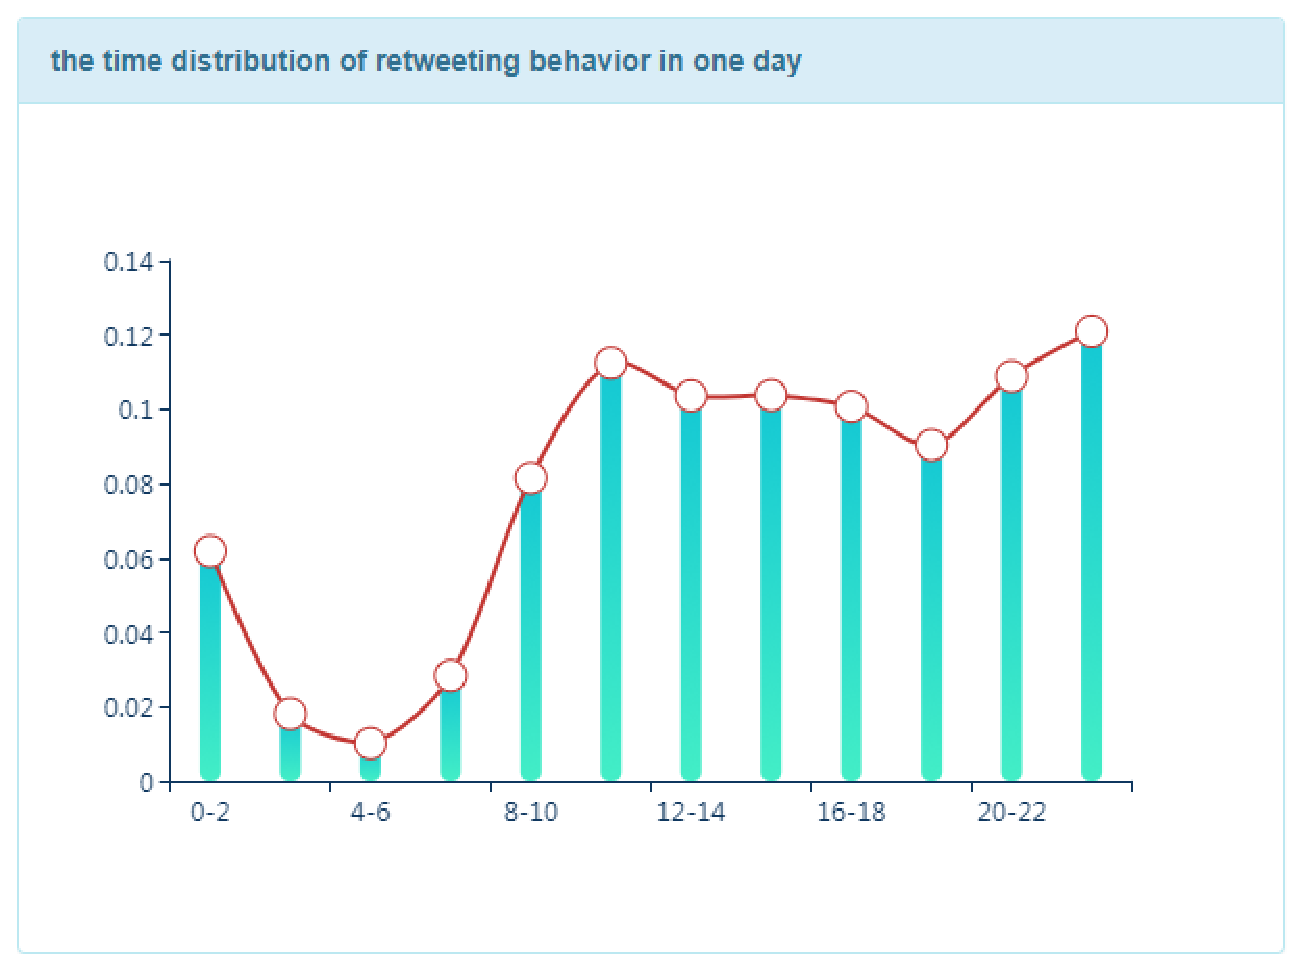
\includegraphics[width=0.23\textwidth]{IMAGE/group-images/26.eps}}
  \subfigure[]{
  \label{fig:subfig2:fig27}
      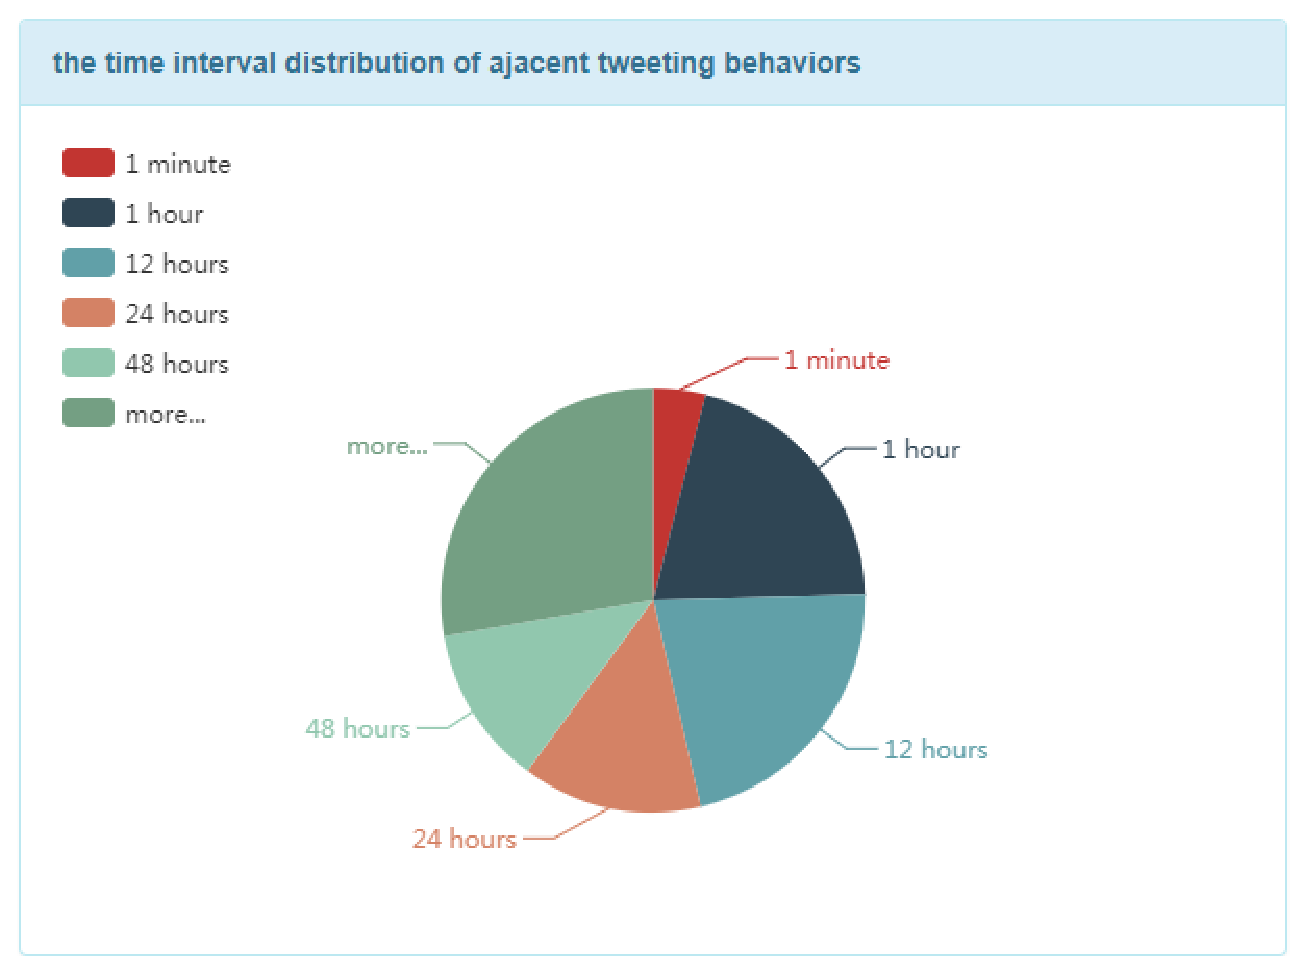
\includegraphics[width=0.23\textwidth]{IMAGE/group-images/27.eps}}
  \subfigure[]{
  \label{fig:subfig2:fig28}
      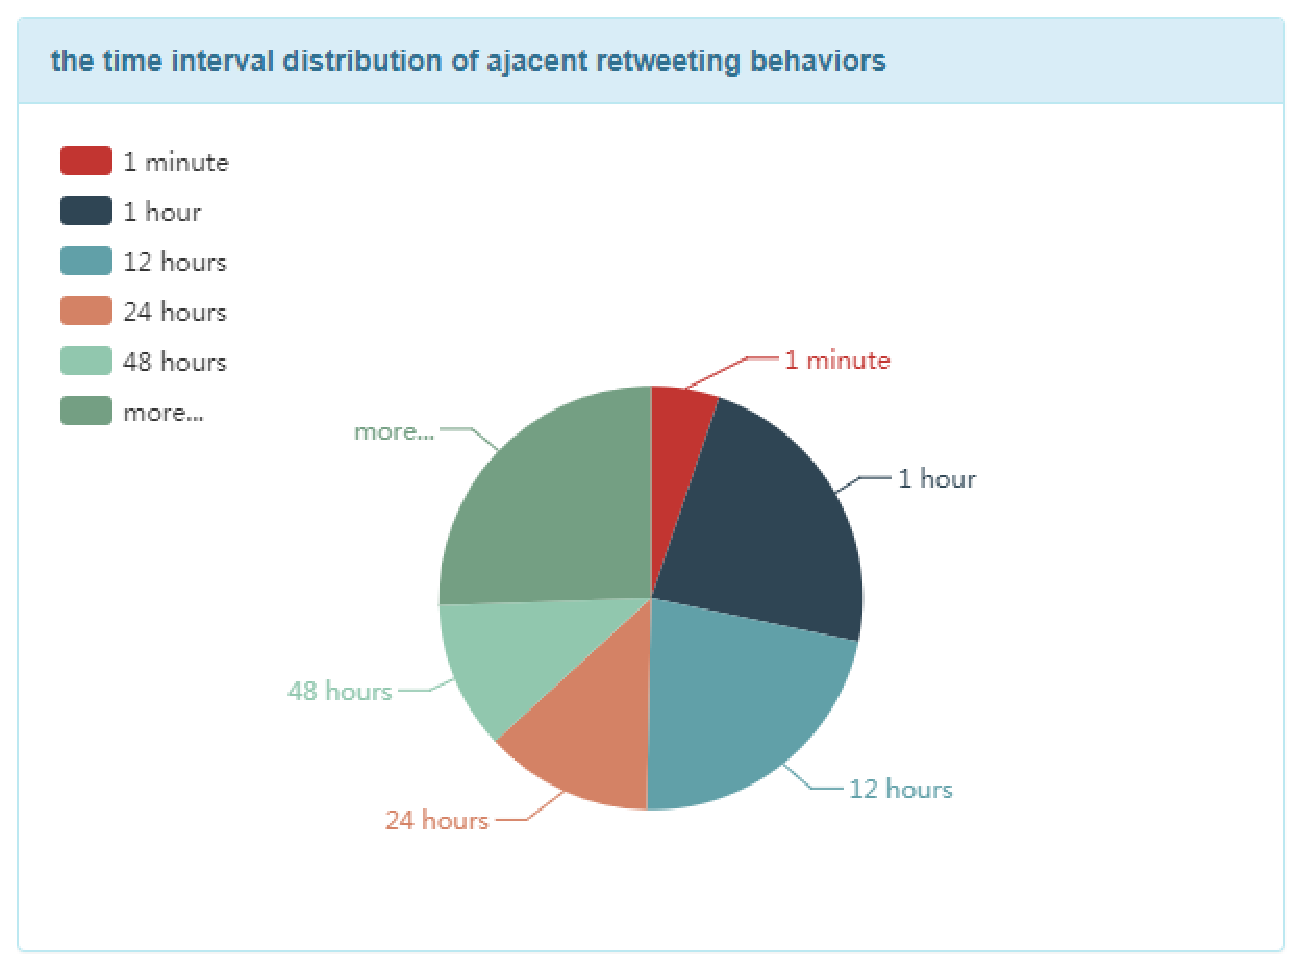
\includegraphics[width=0.23\textwidth]{IMAGE/group-images/28.eps}}
  \subfigure[]{
  \label{fig:subfig2:fig29}
      
\includegraphics[width=0.23\textwidth]{IMAGE/group-images/29.eps}}
  \caption{The Statistics of User Group Two}
  \label{fig:subfig2} %% label for entire figure
\end{figure*}

\begin{figure*}
  \centering
  \subfigure[]{
  \label{fig:subfig3:fig31}
      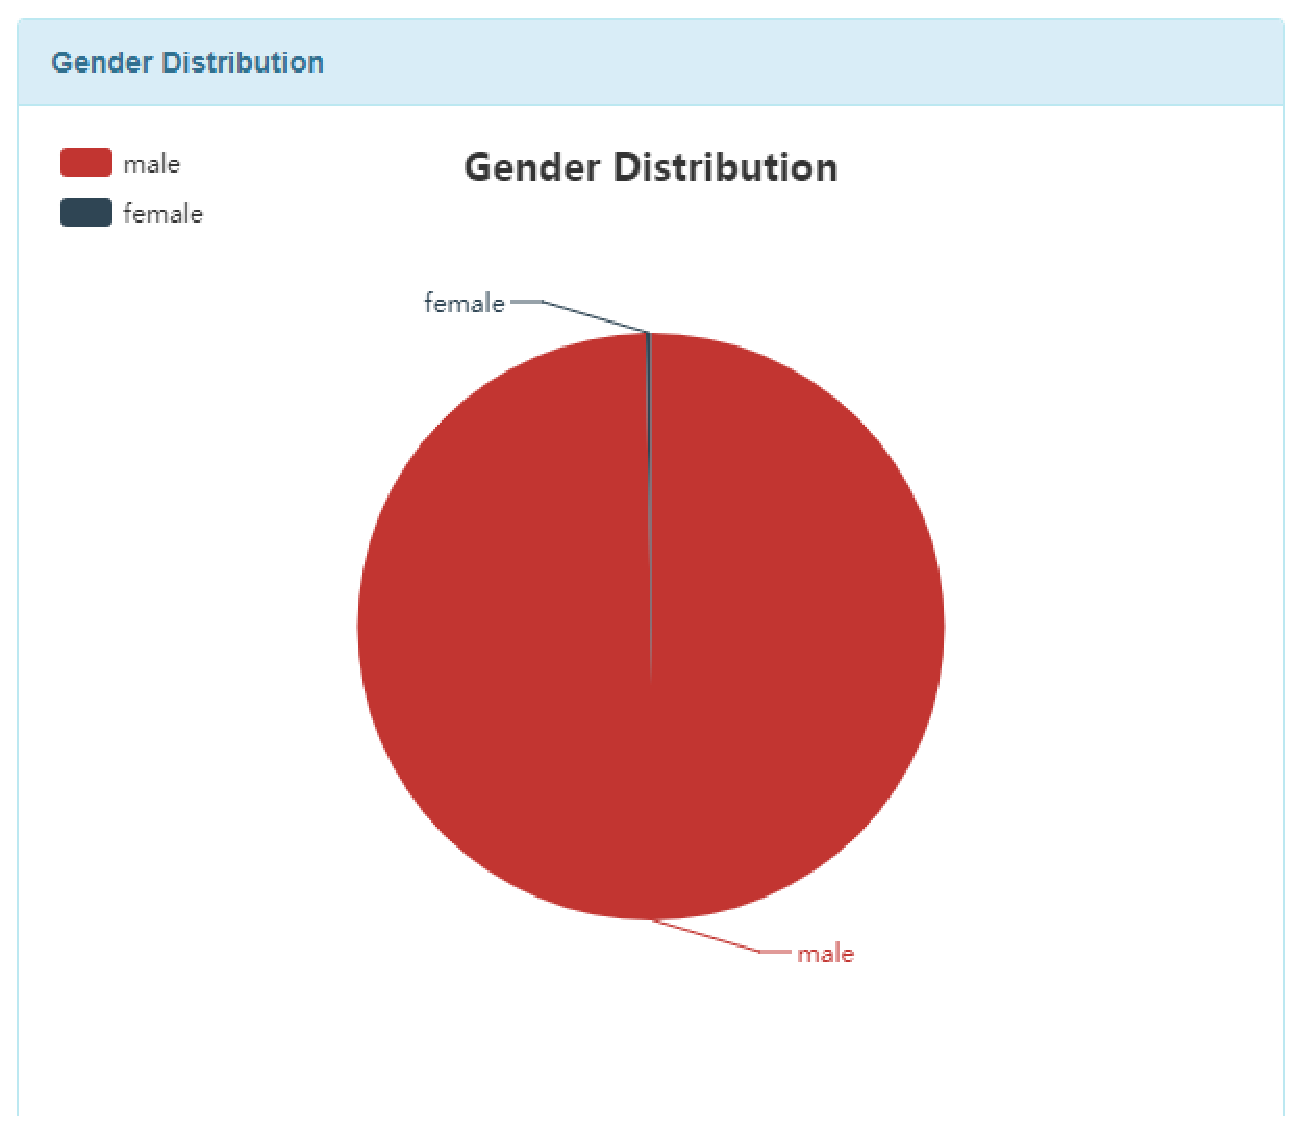
\includegraphics[width=0.23\textwidth]{IMAGE/group-images/31.eps}}
  \subfigure[]{
  \label{fig:subfig3:fig32}
      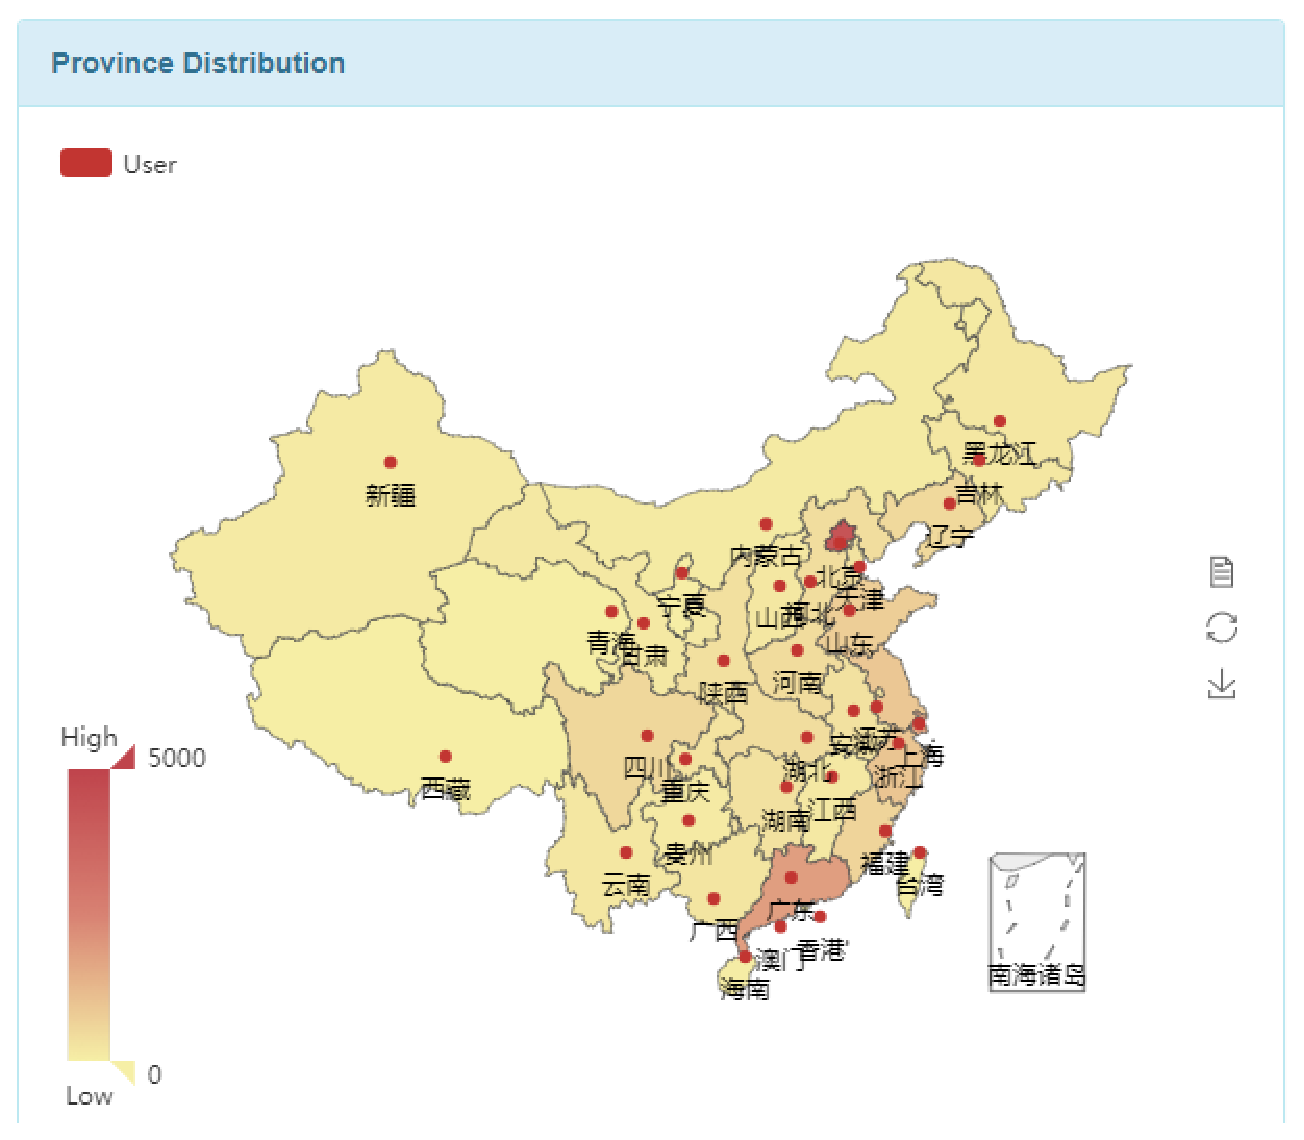
\includegraphics[width=0.23\textwidth]{IMAGE/group-images/32.eps}}
  \subfigure[]{
  \label{fig:subfig3:fig33}
      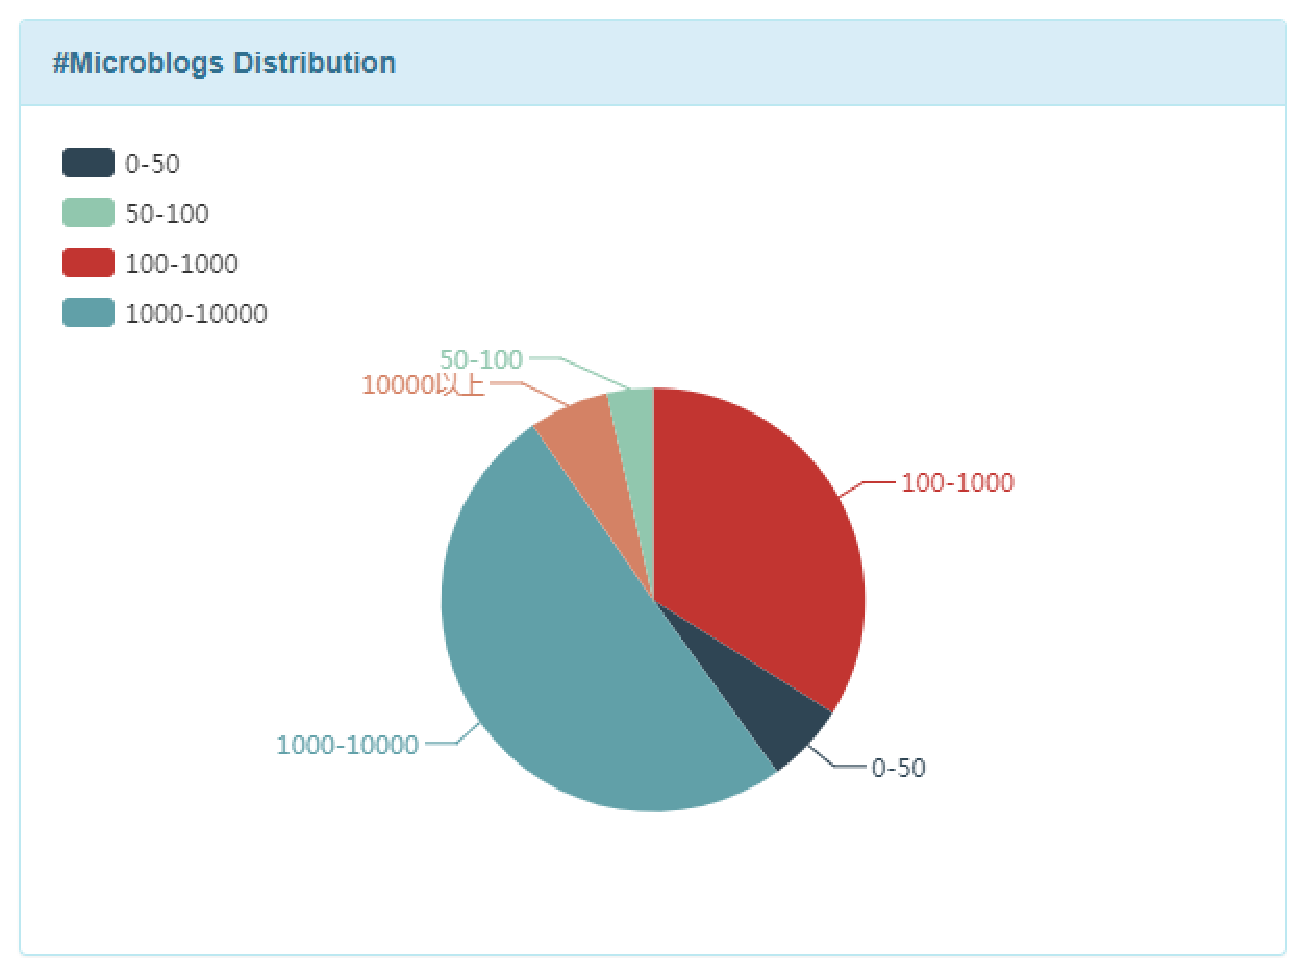
\includegraphics[width=0.23\textwidth]{IMAGE/group-images/33.eps}}
  \subfigure[]{
  \label{fig:subfig3:fig34}
      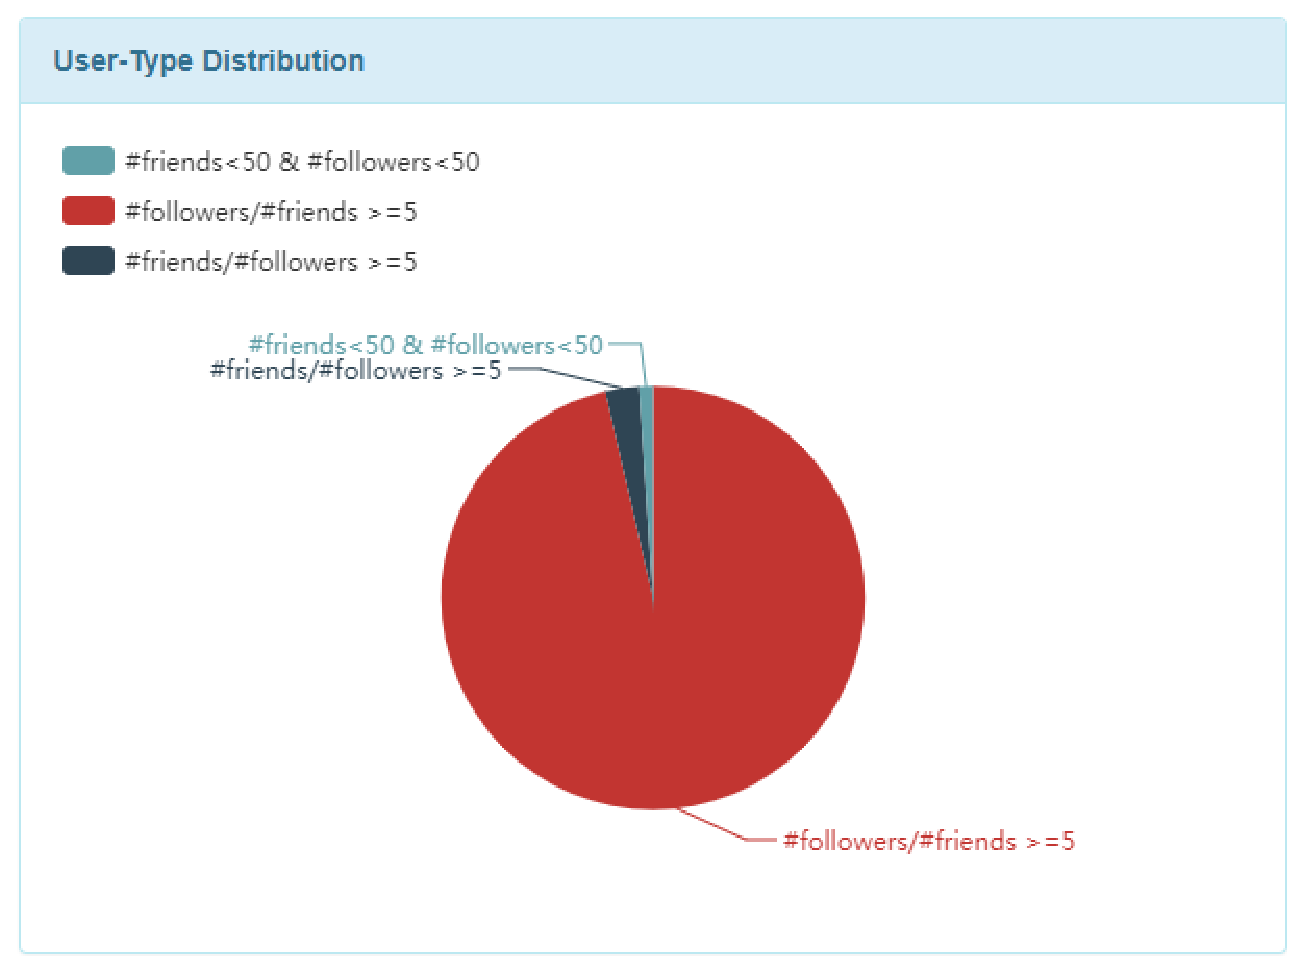
\includegraphics[width=0.23\textwidth]{IMAGE/group-images/34.eps}}
  \subfigure[]{
  \label{fig:subfig3:fig35}
      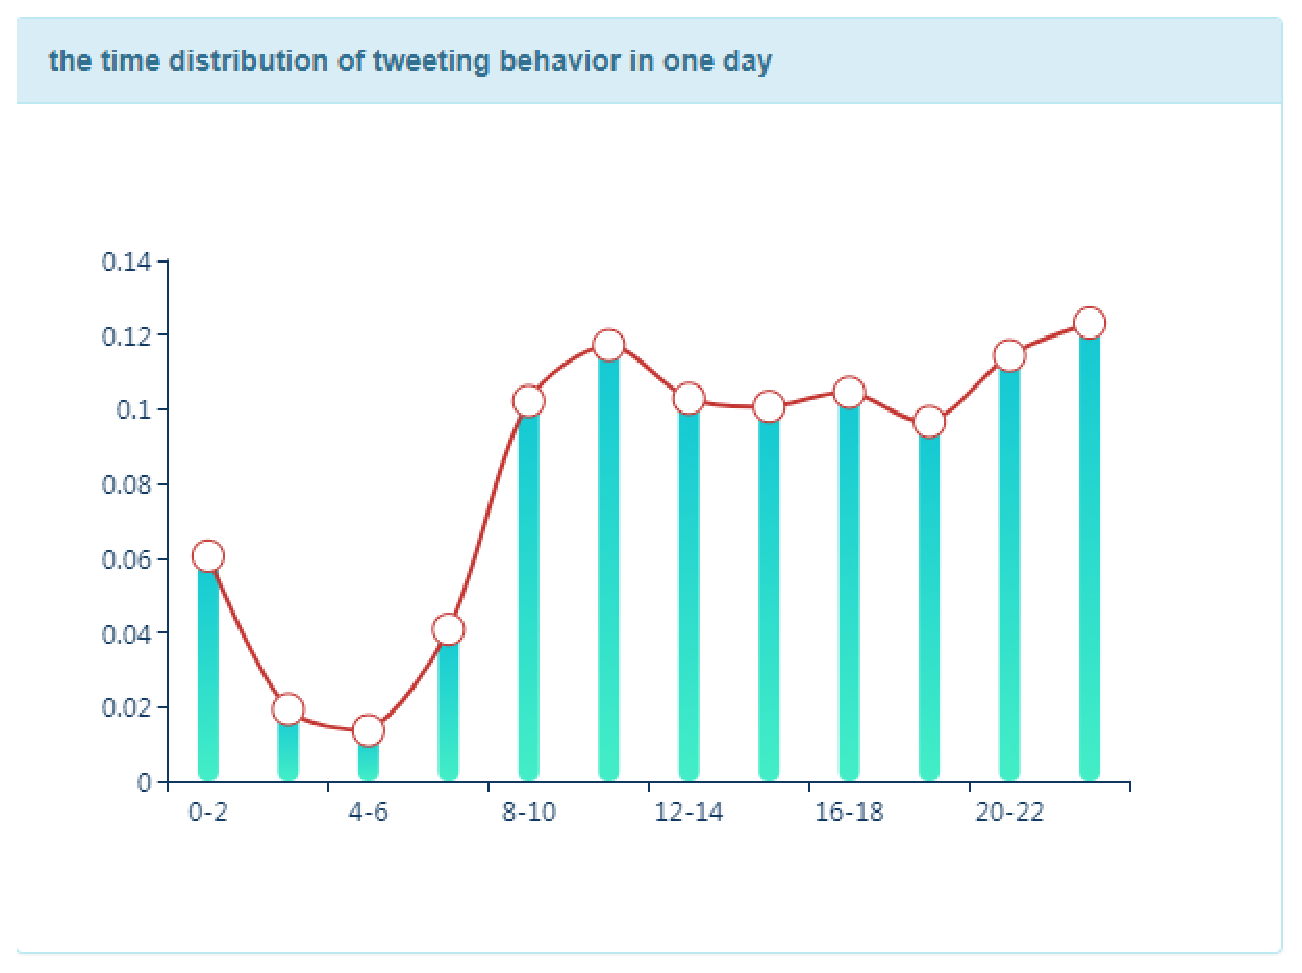
\includegraphics[width=0.23\textwidth]{IMAGE/group-images/35.eps}}
  \subfigure[]{
  \label{fig:subfig3:fig36}
      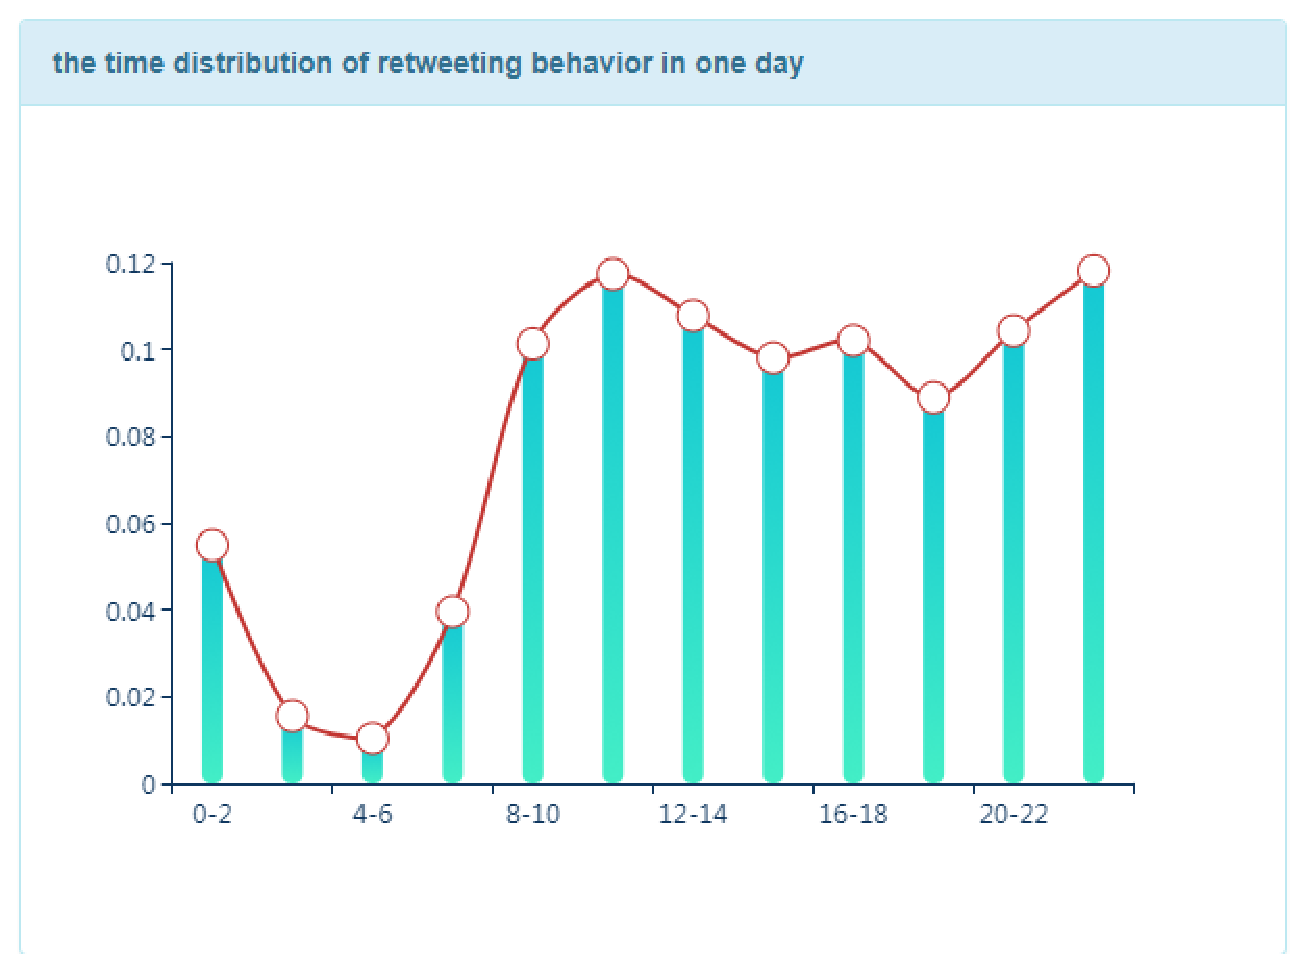
\includegraphics[width=0.23\textwidth]{IMAGE/group-images/36.eps}}
  \subfigure[]{
  \label{fig:subfig3:fig37}
      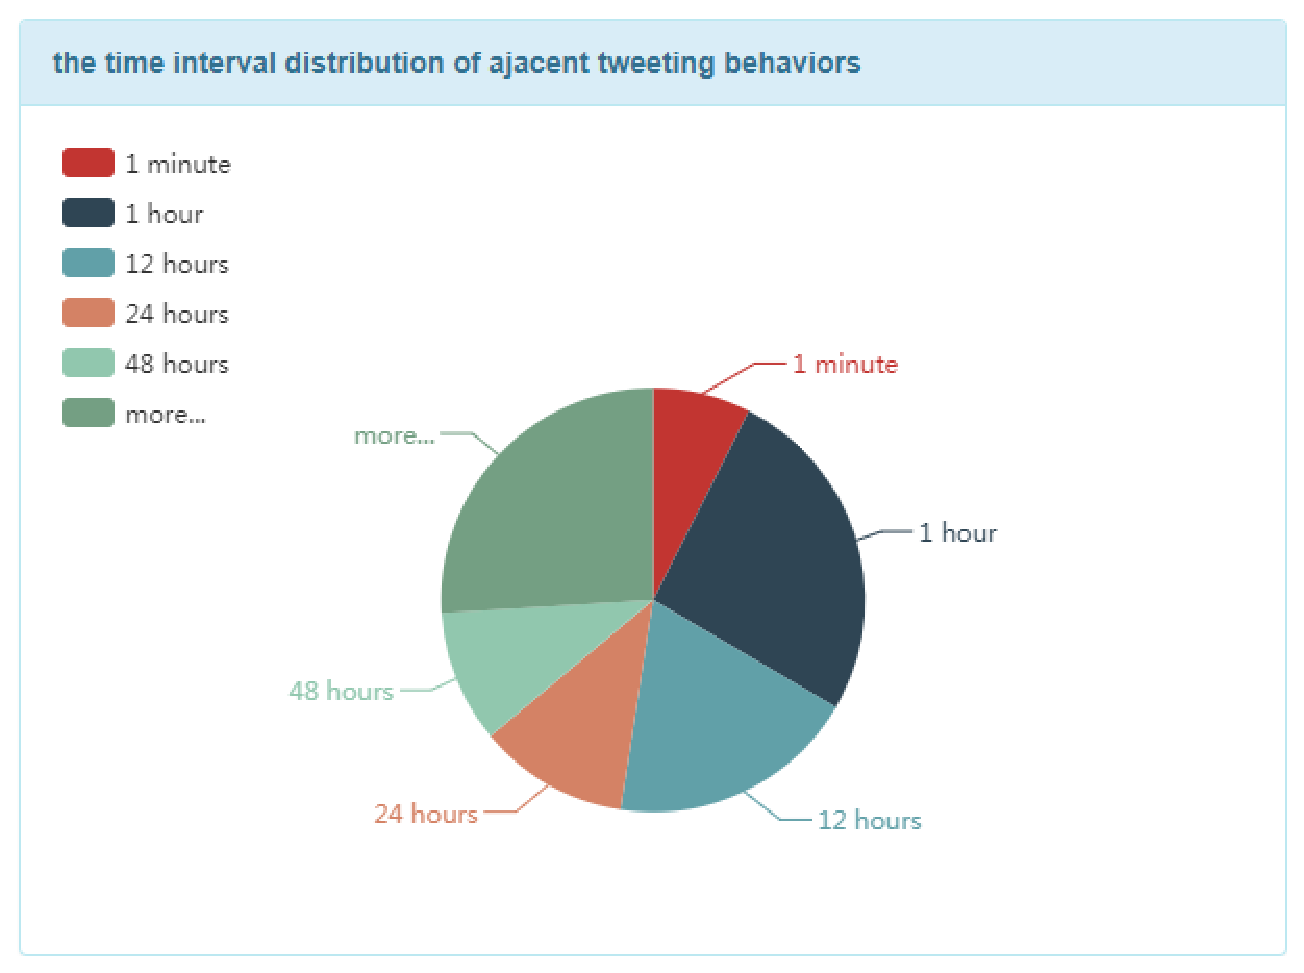
\includegraphics[width=0.23\textwidth]{IMAGE/group-images/37.eps}}
  \subfigure[]{
  \label{fig:subfig3:fig38}
      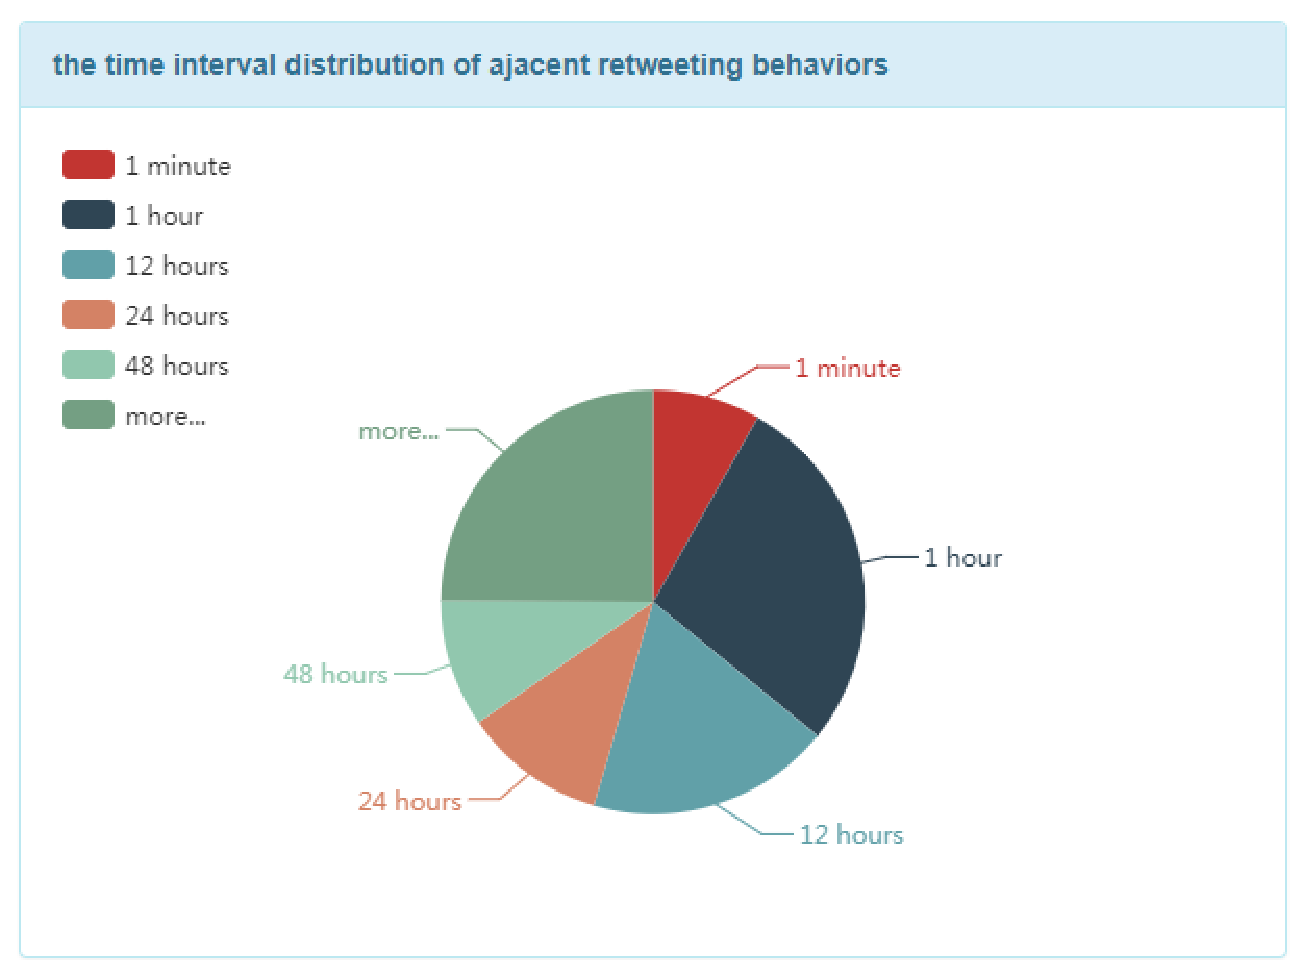
\includegraphics[width=0.23\textwidth]{IMAGE/group-images/38.eps}}
  \subfigure[]{
  \label{fig:subfig3:fig39}
      
\includegraphics[width=0.23\textwidth]{IMAGE/group-images/39.eps}}
  \caption{The Statistics of User Group Three}
  \label{fig:subfig3} %% label for entire figure
\end{figure*}


\begin{figure*}
  \centering
  \subfigure[]{
  \label{fig:subfig4:fig41}
      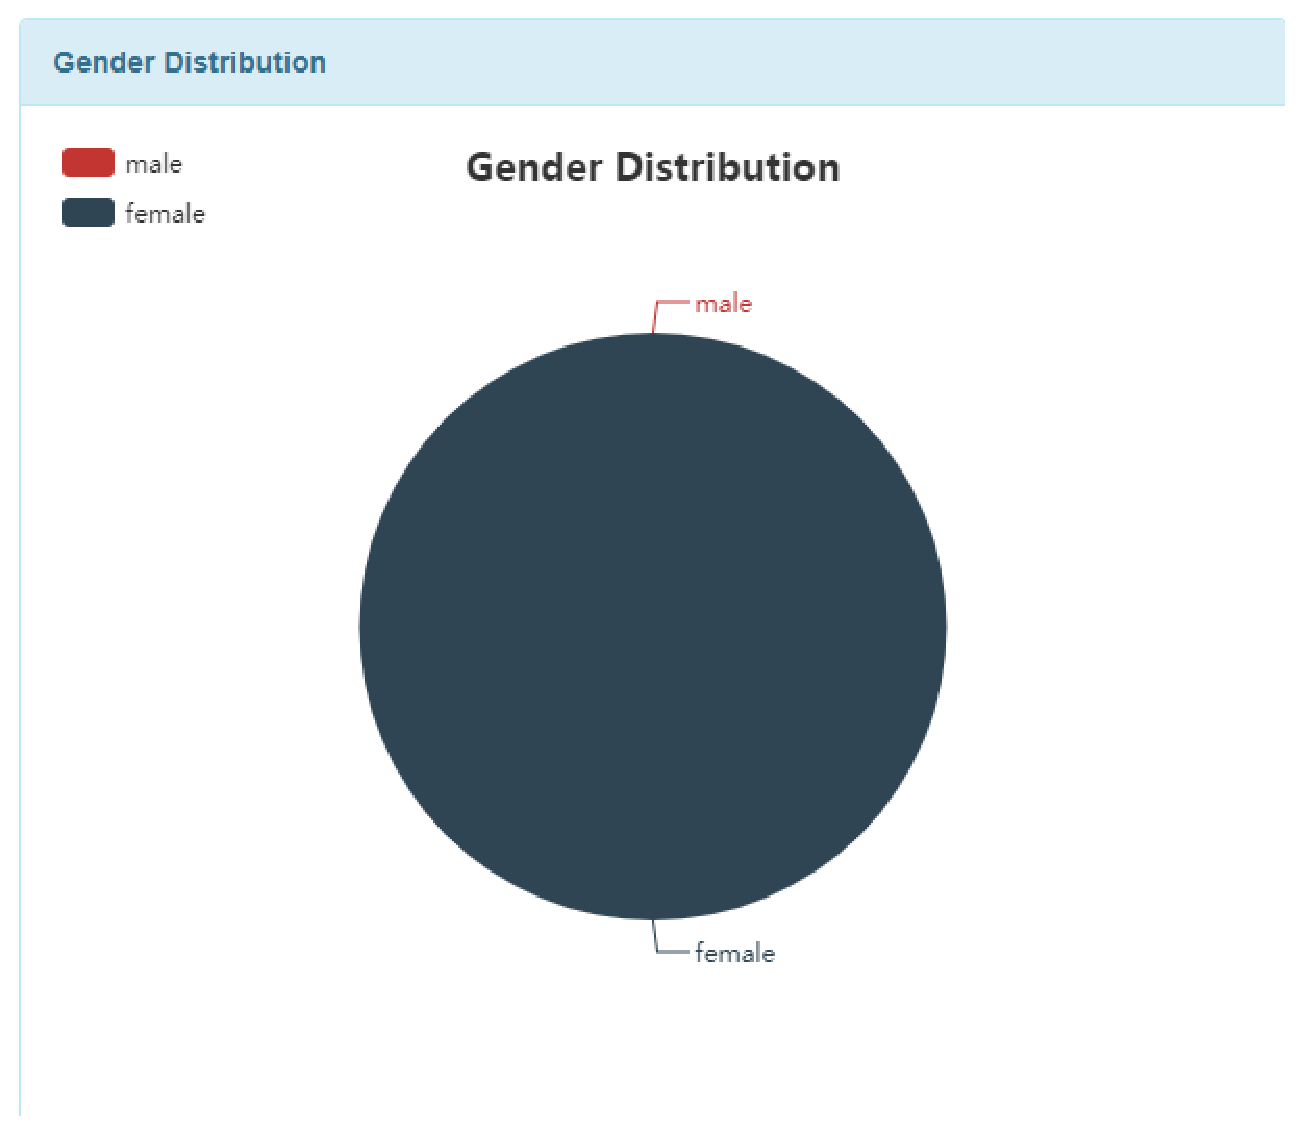
\includegraphics[width=0.23\textwidth]{IMAGE/group-images/41.eps}}
  \subfigure[]{
  \label{fig:subfig4:fig42}
      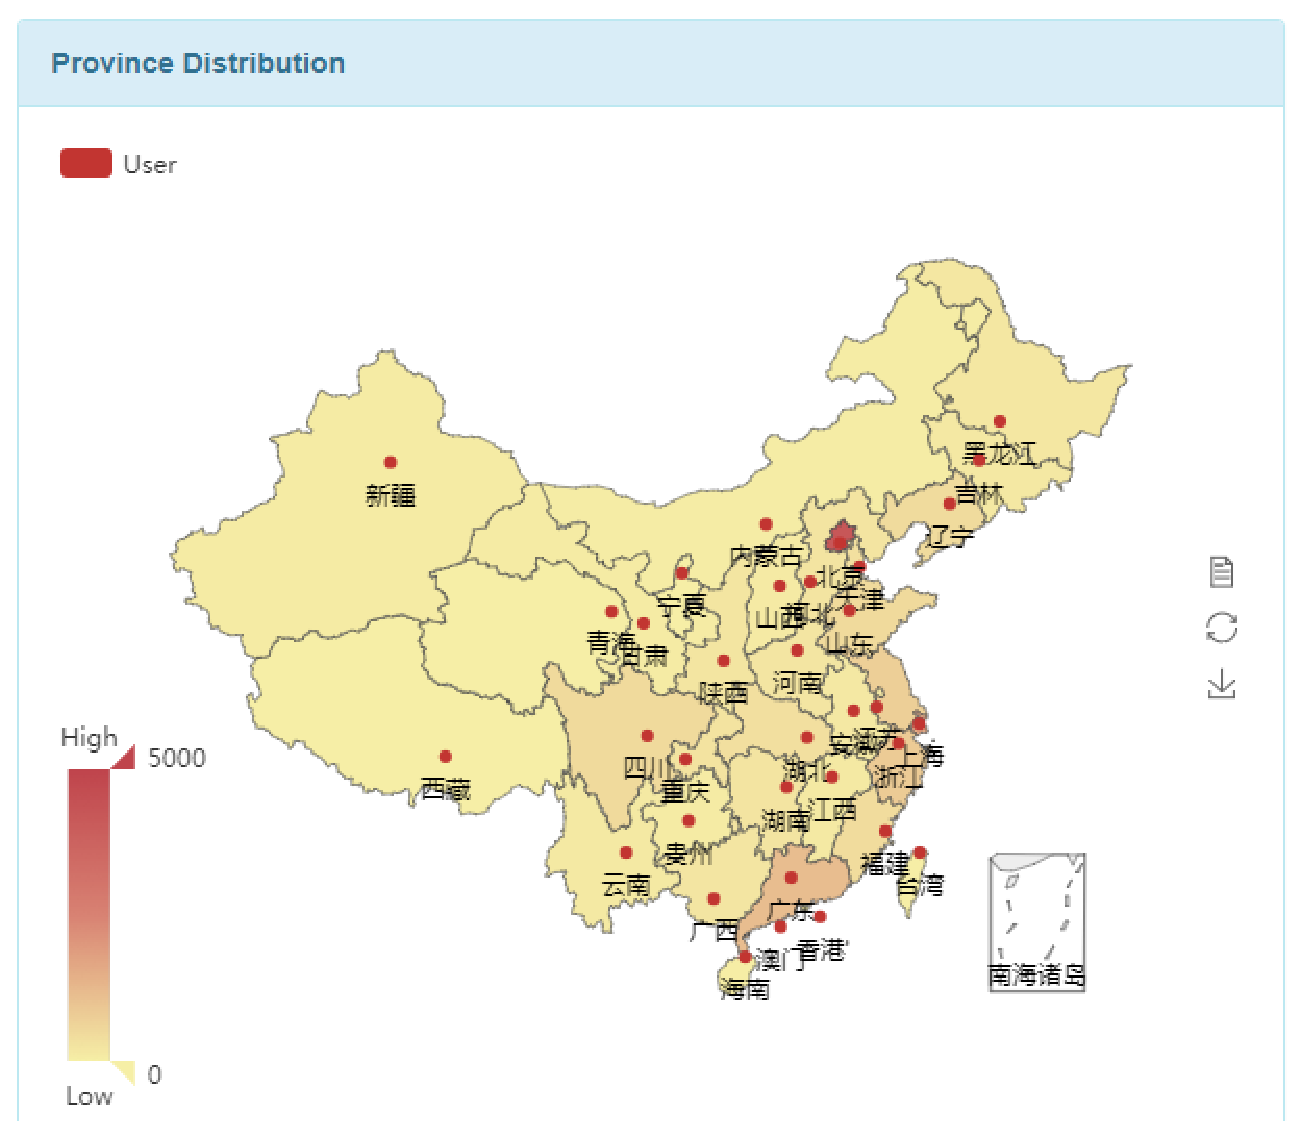
\includegraphics[width=0.23\textwidth]{IMAGE/group-images/42.eps}}
  \subfigure[]{
  \label{fig:subfig4:fig43}
      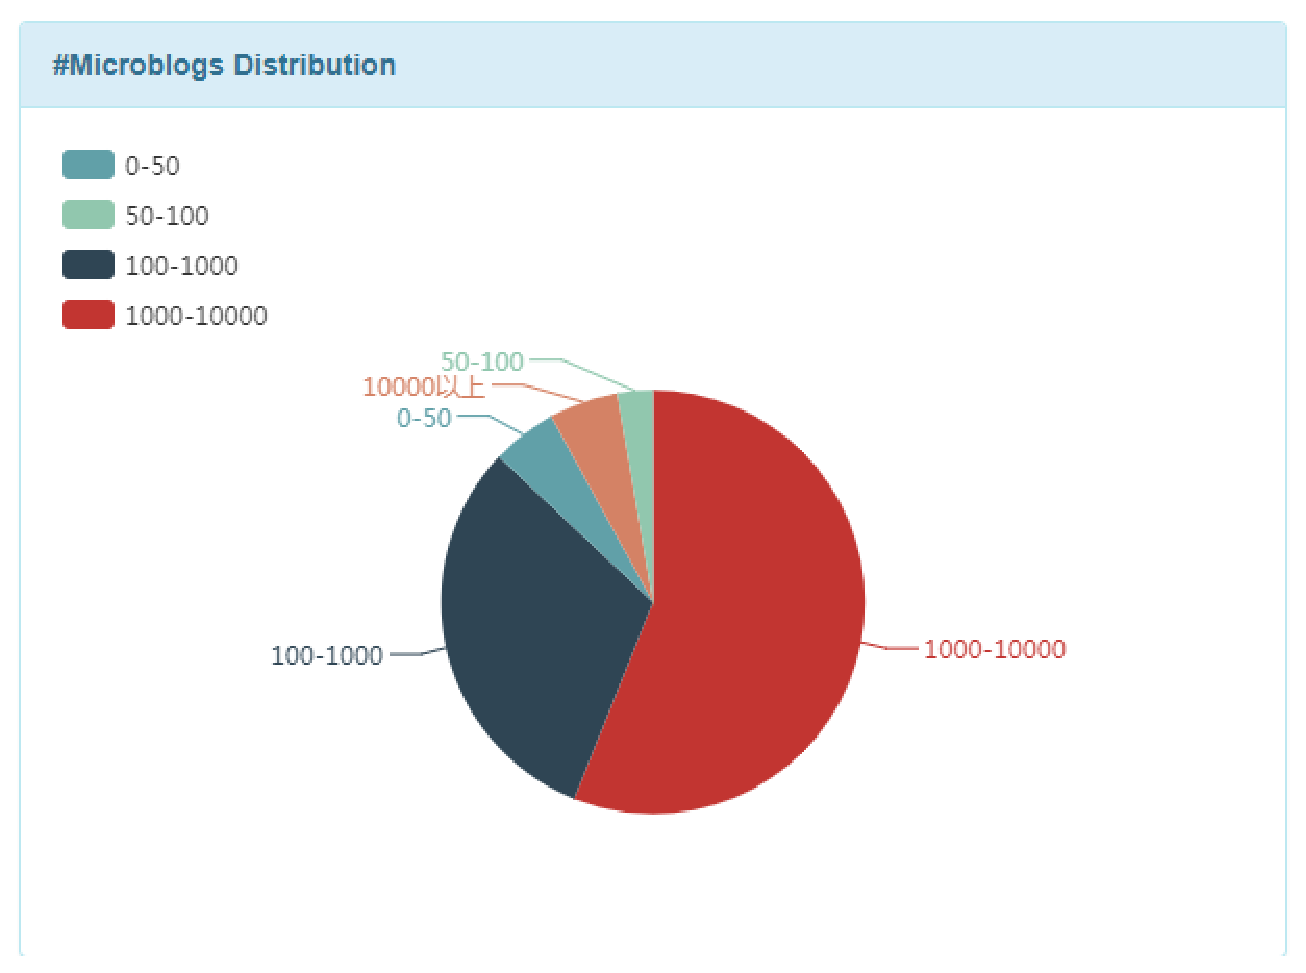
\includegraphics[width=0.23\textwidth]{IMAGE/group-images/43.eps}}
  \subfigure[]{
  \label{fig:subfig4:fig44}
      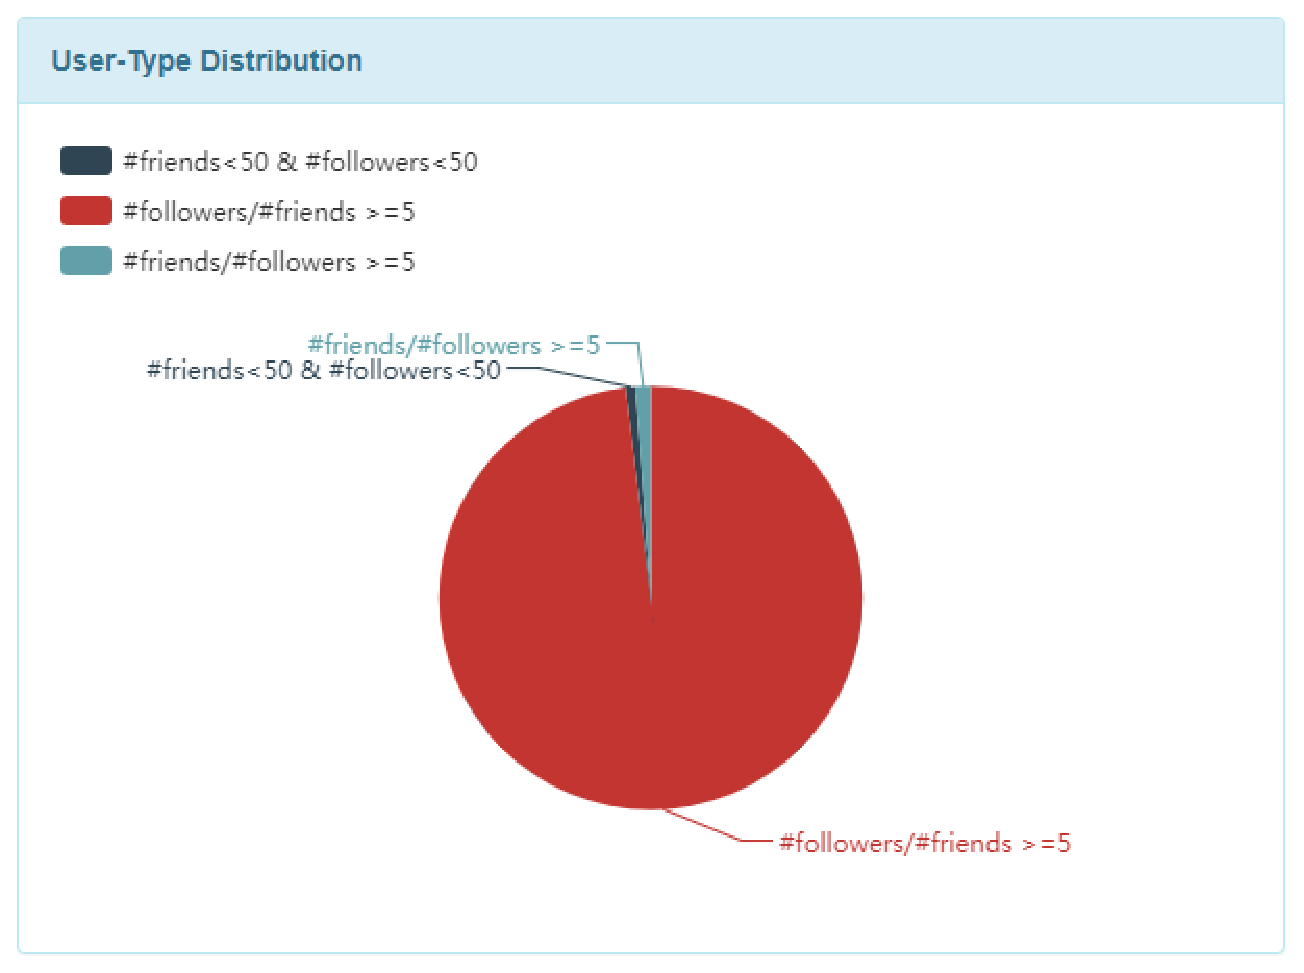
\includegraphics[width=0.23\textwidth]{IMAGE/group-images/44.eps}}
  \subfigure[]{
  \label{fig:subfig4:fig45}
      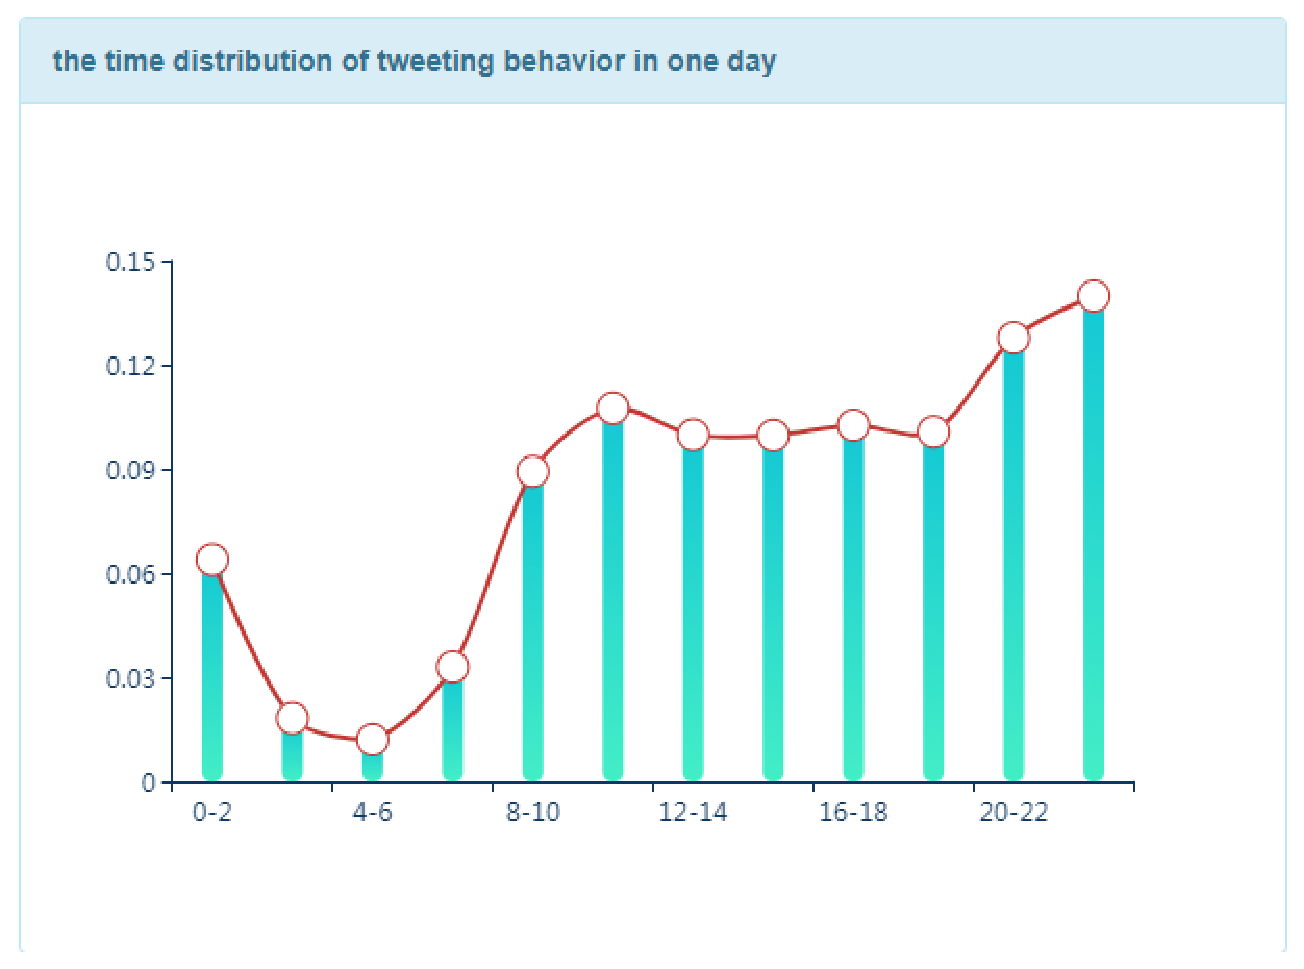
\includegraphics[width=0.23\textwidth]{IMAGE/group-images/45.eps}}
  \subfigure[]{
  \label{fig:subfig4:fig46}
      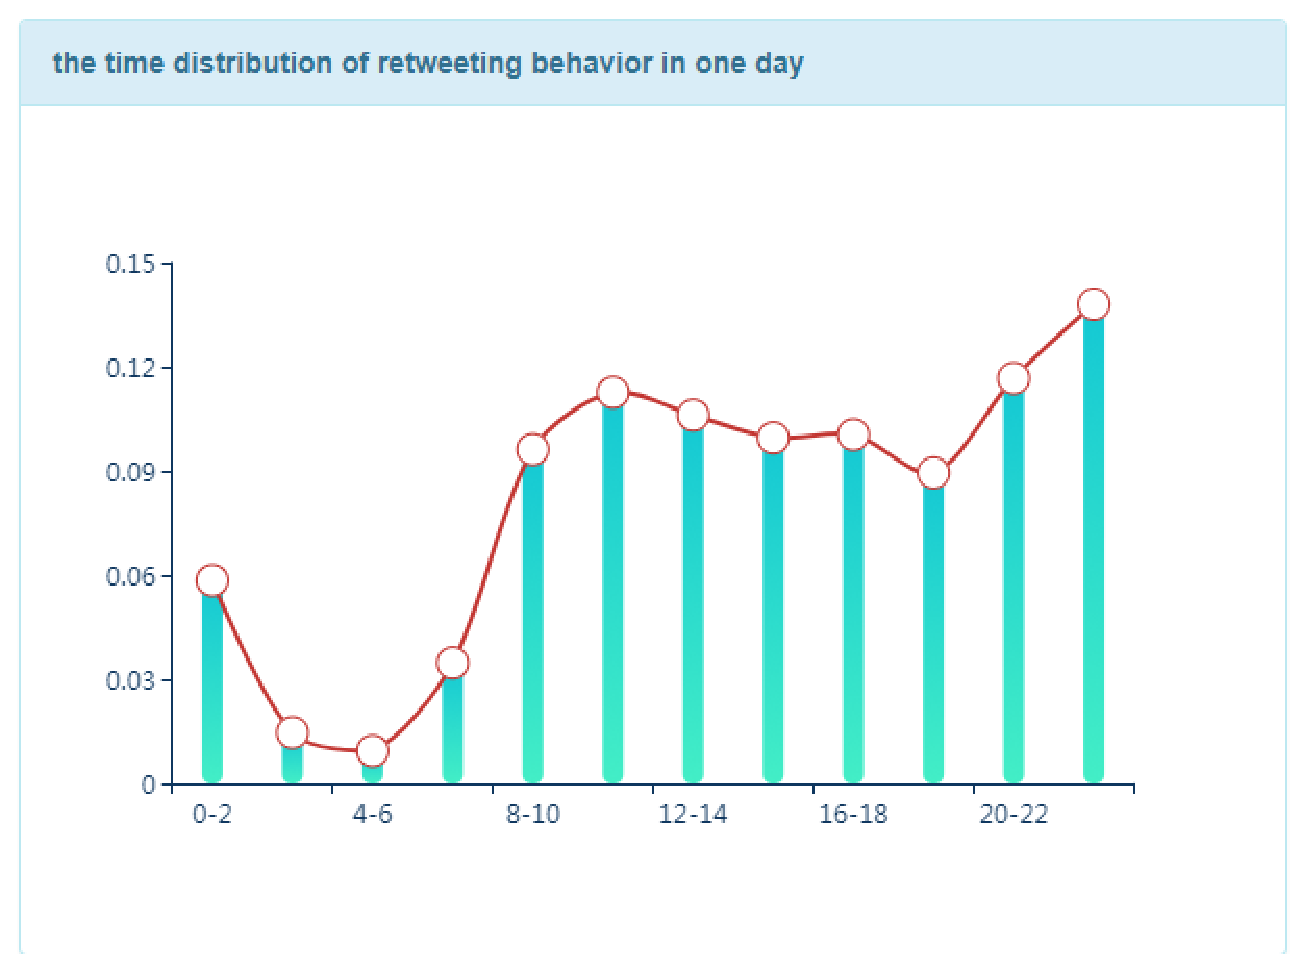
\includegraphics[width=0.23\textwidth]{IMAGE/group-images/46.eps}}
  \subfigure[]{
  \label{fig:subfig4:fig47}
      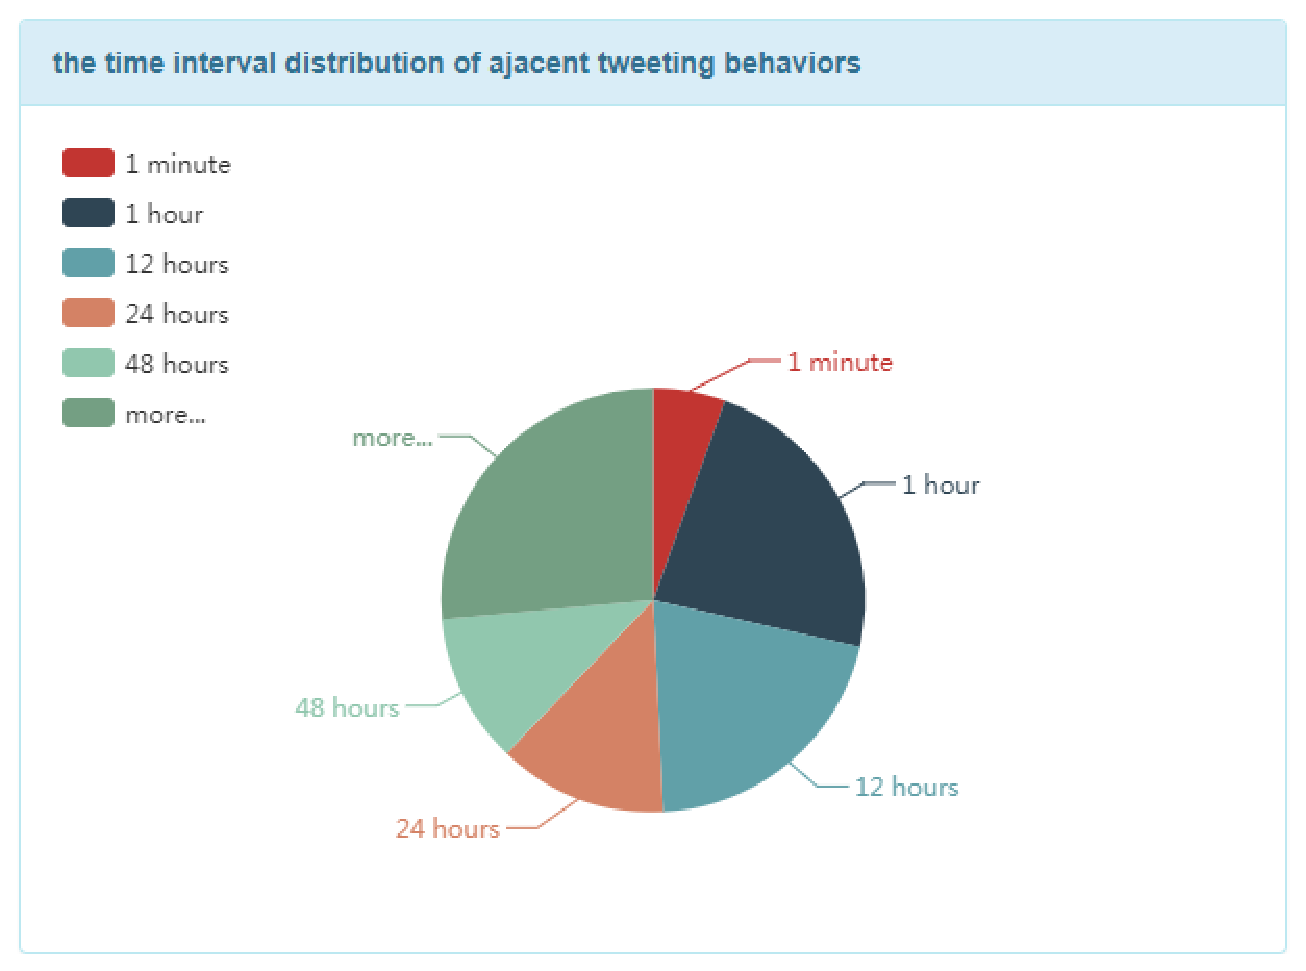
\includegraphics[width=0.23\textwidth]{IMAGE/group-images/47.eps}}
  \subfigure[]{
  \label{fig:subfig4:fig48}
      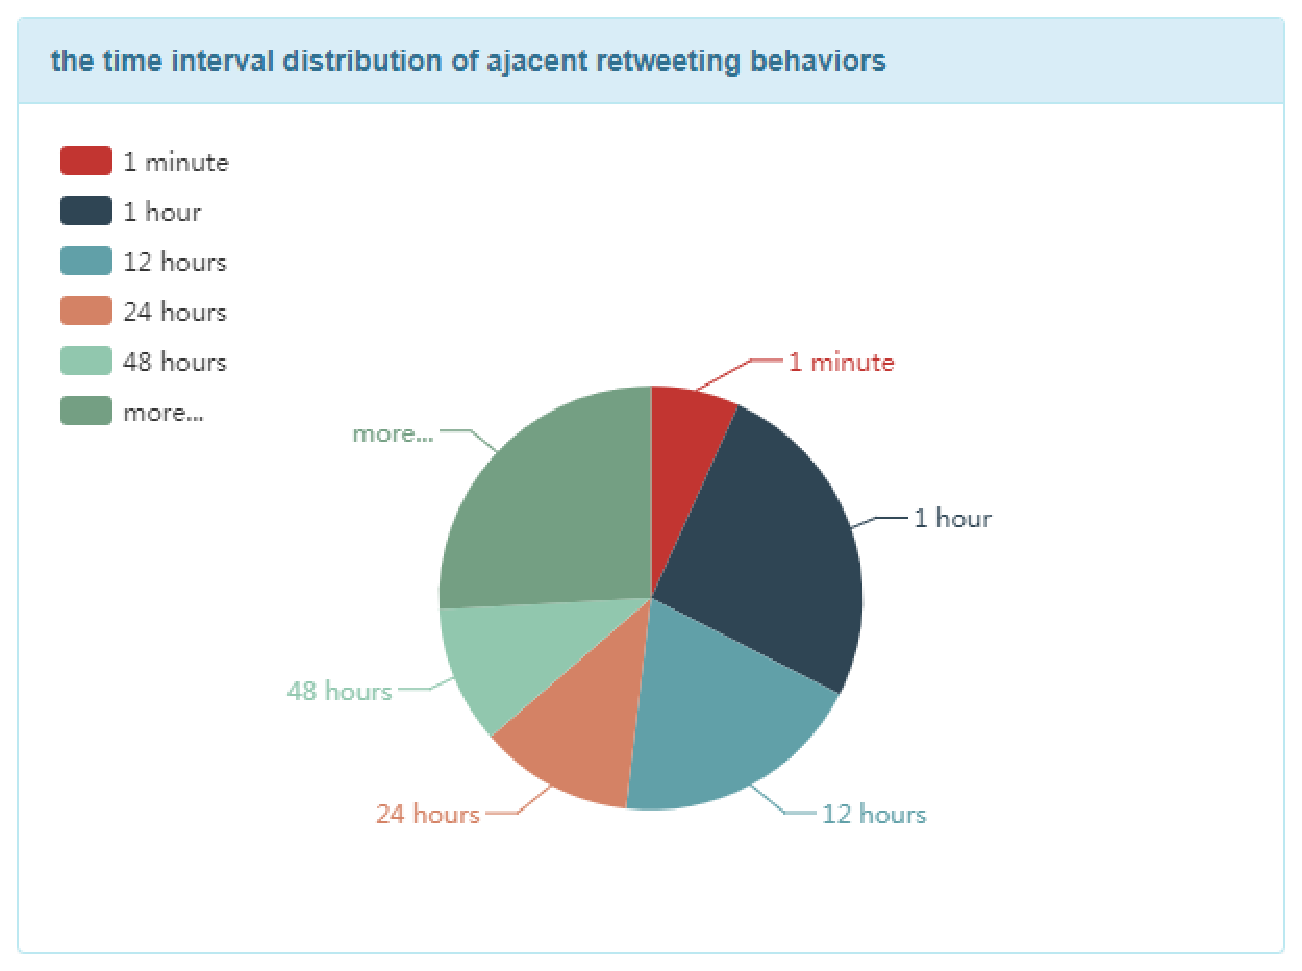
\includegraphics[width=0.23\textwidth]{IMAGE/group-images/48.eps}}
  \subfigure[]{
  \label{fig:subfig4:fig49}
      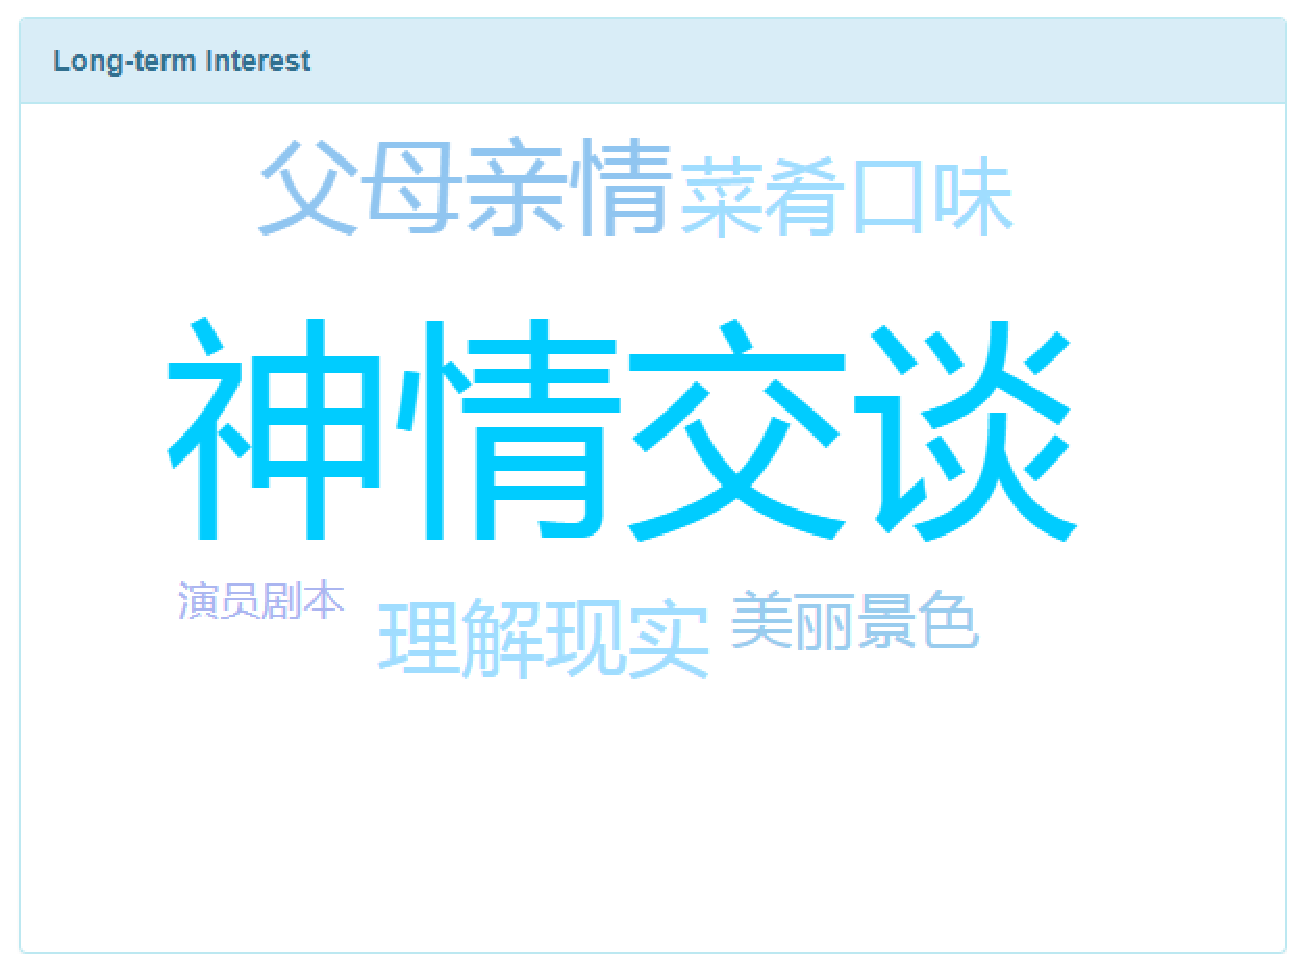
\includegraphics[width=0.23\textwidth]{IMAGE/group-images/49.eps}}
  \caption{The Statistics of User Group Four}
  \label{fig:subfig4} %% label for entire figure
\end{figure*}


\end{CJK*}
\end{document}

% End of ltexpprt.tex
